% !TeX root = ../main.tex

%%% Tables %%%

\begin{table}[ht]
\centering
\caption{Estimates and standard errors for the parameters of the distribution of dive duration $(Y_t)$, acceleration $(\Zone_{t,\tilde t^*})$, and ``wiggliness" $(\Ztwo_{t,\tilde t^*})$ of the killer whale kinematic data using the full CarHHMM-DFT. Figures following $\pm$ refer to standard errors estimated using the observed information matrix.}
\scalebox{0.825}{
    \begin{tabular}{ccccc}
        \multirow{2}{*}{Feature}                                                       & \multirow{2}{*}{Dive type / subdive state} & \multicolumn{3}{c}{Parameter estimate}        \\
                                                                                       &                                      & $\hat \mu$    & $\hat \sigma$ & $\hat \phi$   \\ \hline
        \multirow{2}{*}{Dive Duration $(s)$ -- $Y_t$}                                  & 1                                    & $27.342 \pm 0.633$ & $10.961 \pm 0.560$ & ---           \\
                                                                                       & 2                                    & $127.548 \pm 11.341$ & $63.888 \pm 9.032$ & ---           \\ \hline
        \multirow{3}{*}{$x$-Acc. $(m/s^2)$ -- $\left(\Zone_{t,\tilde t^*}\right)_x$}   & 1                                    & $0.449 \pm 0.030$ & $0.039 \pm 0.001$ & $0.968 \pm 0.002$ \\
                                                                                       & 2                                    & $0.210 \pm 0.012$ & $0.096 \pm 0.002$ & $0.829 \pm 0.007$ \\
                                                                                       & 3                                    & $0.232 \pm 0.035$ & $0.296 \pm 0.010$ & $0.607 \pm 0.023$ \\ \hline
        \multirow{3}{*}{$y$-Acc. $(m/s^2)$ -- $\left(\Zone_{t,\tilde t^*}\right)_y$}   & 1                                    & $0.450 \pm 0.038$ & $0.051 \pm 0.001$ & $0.968 \pm 0.002$ \\
                                                                                       & 2                                    & $0.437 \pm 0.012$ & $0.094 \pm 0.002$ & $0.829 \pm 0.007$ \\
                                                                                       & 3                                    & $0.366 \pm 0.042$ & $0.365 \pm 0.012$ & $0.607 \pm 0.023$ \\ \hline
        \multirow{3}{*}{$z$-Acc. $(m/s^2)$ -- $\left(\Zone_{t,\tilde t^*}\right)_z$}   & 1                                    & $-0.691 \pm 0.043$ & $0.058 \pm 0.001$ & $0.968 \pm 0.002$ \\
                                                                                       & 2                                    & $-0.573 \pm 0.014$ & $0.111 \pm 0.002$ & $0.829 \pm 0.007$ \\
                                                                                       & 3                                    & $-0.303 \pm 0.041$ & $0.354 \pm 0.012$ & $0.607 \pm 0.023$ \\ \hline
        \multirow{3}{*}{Wiggliness -- $\Ztwo_{t,\tilde t^*}$}                          & 1                                    & $34.015 \pm 0.368$ & $22.986 \pm 0.378$ & ---           \\
                                                                                       & 2                                    & $490.068 \pm 5.584$ & $502.558 \pm 6.776$ & ---           \\
                                                                                       & 3                                    & $9154.156 \pm 220.765$ & $13538.747 \pm 354.281$ & ---           \\ \hline
    \end{tabular}
    }
    \label{table:emis_dists_CarHHMM-DFT}
\end{table}

\begin{table}[ht]
\centering
\caption{Average decoding accuracies and training times for all models in the simulation study. Each of the four models was fit to 500 training data sets composed of 100 simulated dives and tested on test data sets also composed of 100 simulated dives. Reported values are averages, and figures following $\pm$ refer to sample standard deviation across the 500 data sets. ``All" denotes overall average decoding accuracy.}
\scalebox{0.9}{
\begin{tabular}{ccccccc}
Model                       & \multicolumn{1}{c}{Training time ($min$)} & \multicolumn{1}{c}{Dive type} & \multicolumn{1}{c}{Subdive type} & \multicolumn{1}{c}{Dive accuracy} & \multicolumn{1}{c}{Subdive accuracy}  \\ \hline
\multirow{7}{*}{CarHHMM-DFT}& \multirow{7}{*}{$156 \pm 67$}   & All                           & All                              & $0.956 \pm 0.028$                   & $0.911 \pm 0.006$                       \\
                            &                                    & 1                             & 1                                & \multirow{3}{*}{$0.973\pm0.032$}    & $0.846 \pm 0.027$                       \\
                            &                                    & 1                             & 2                                &                                   & $0.918 \pm 0.011$                       \\ 
                            &                                    & 1                             & 3                                &                                   & $0.860 \pm 0.030$                       \\ 
                            &                                    & 2                             & 1                                & \multirow{3}{*}{$0.856\pm0.097$}    & $0.949 \pm 0.010$                       \\ 
                            &                                    & 2                             & 2                                &                                   & $0.915 \pm 0.015$                       \\
                            &                                    & 2                             & 3                                &                                   & $0.871 \pm 0.057$                       \\ \hline
\multirow{7}{*}{HHMM-DFT}   & \multirow{7}{*}{$162 \pm 64$}   & All                           & All                              & $0.959 \pm 0.025$                   & $0.844 \pm 0.024$                       \\
                            &                                    & 1                             & 1                                & \multirow{3}{*}{$0.977\pm0.028$}    & $0.761 \pm 0.063$                       \\ 
                            &                                    & 1                             & 2                                &                                   & $0.845 \pm 0.029$                       \\ 
                            &                                    & 1                             & 3                                &                                   & $0.858 \pm 0.034$                       \\
                            &                                    & 2                             & 1                                & \multirow{3}{*}{$0.851\pm0.097$}    & $0.883 \pm 0.066$                       \\ 
                            &                                    & 2                             & 2                                &                                   & $0.829 \pm 0.041$                       \\
                            &                                    & 2                             & 3                                &                                   & $0.876 \pm 0.061$                       \\ \hline
\multirow{7}{*}{CarHHMM}    & \multirow{7}{*}{$258 \pm 106$}   & All                           & All                              & $0.924 \pm 0.127$                   & $0.845 \pm 0.018$                       \\
                            &                                    & 1                             & 1                                & \multirow{3}{*}{$0.933\pm0.153$}    & $0.689 \pm 0.050$                       \\ 
                            &                                    & 1                             & 2                                &                                   & $0.900 \pm 0.031$                       \\ 
                            &                                    & 1                             & 3                                &                                   & $0.673 \pm 0.059$                       \\
                            &                                    & 2                             & 1                                & \multirow{3}{*}{$0.864\pm0.134$}    & $0.906 \pm 0.022$                       \\ 
                            &                                    & 2                             & 2                                &                                   & $0.848 \pm 0.033$                       \\
                            &                                    & 2                             & 3                                &                                   & $0.687 \pm 0.105$                       \\ \hline
\multirow{7}{*}{CarHMM-DFT} & \multirow{7}{*}{$45 \pm 22$}   & All                           & All                              & ---                                   & $0.912 \pm 0.006$                       \\
                            &                                    & 1                             & 1                                & \multirow{3}{*}{---          }    & $0.854 \pm 0.026$                       \\
                            &                                    & 1                             & 2                                &                                   & $0.921 \pm 0.011$                       \\                            
                            &                                    & 1                             & 3                                &                                   & $0.860 \pm 0.032$                       \\ 
                            &                                    & 2                             & 1                                & \multirow{3}{*}{---          }    & $0.943 \pm 0.011$                       \\ 
                            &                                    & 2                             & 2                                &                                   & $0.919 \pm 0.014$                       \\ 
                            &                                    & 2                             & 3                                &                                   & $0.878 \pm 0.053$                       \\ \hline
\end{tabular}
}

\label{table:accuracy}
\end{table}

%%% model definitions %%%

\begin{figure}[ht]
    \begin{subfigure}{\textwidth}
      \centering
      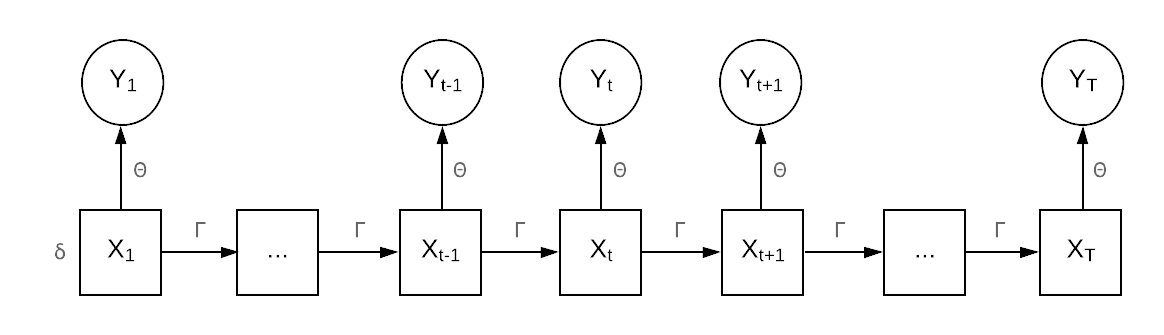
\includegraphics[width=3.5in]{../Plots/HMM.png}  
      \label{fig:HMM}
    \end{subfigure}
    %
    \hrule
    %
    \begin{subfigure}{\textwidth}
      \centering
      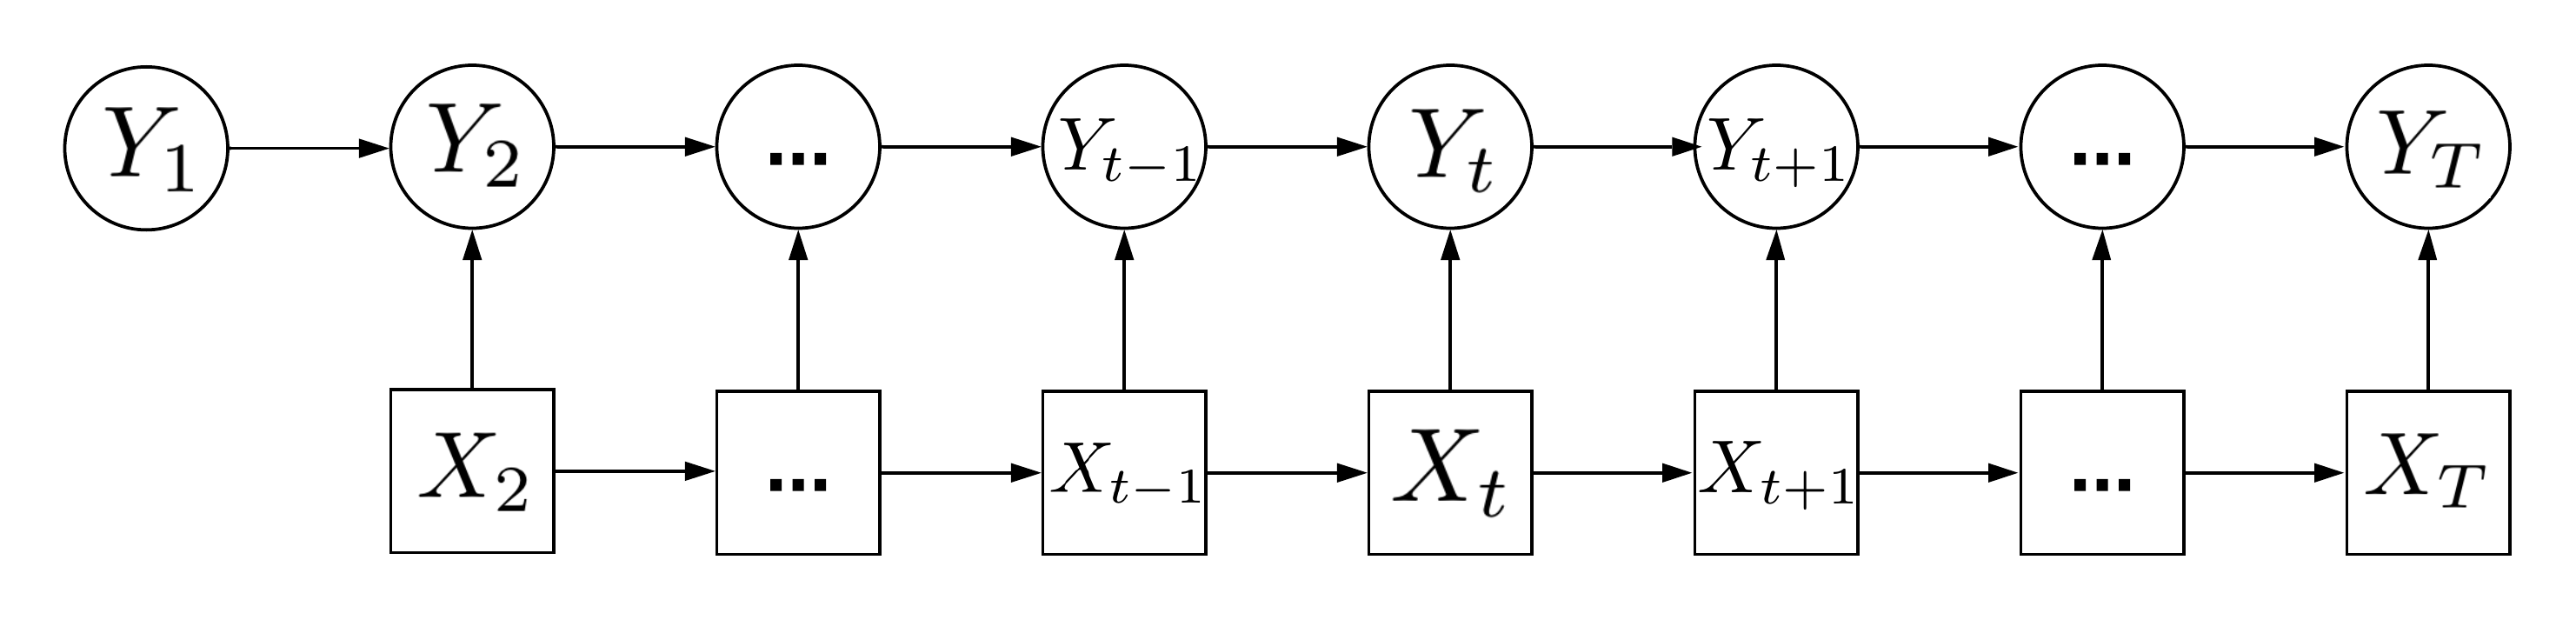
\includegraphics[width=3.5in]{../Plots/CarHMM.png}  
      \label{fig:CarHMM}
    \end{subfigure}
    %
    \hrule
    %
    \begin{subfigure}{\textwidth}
      \centering
      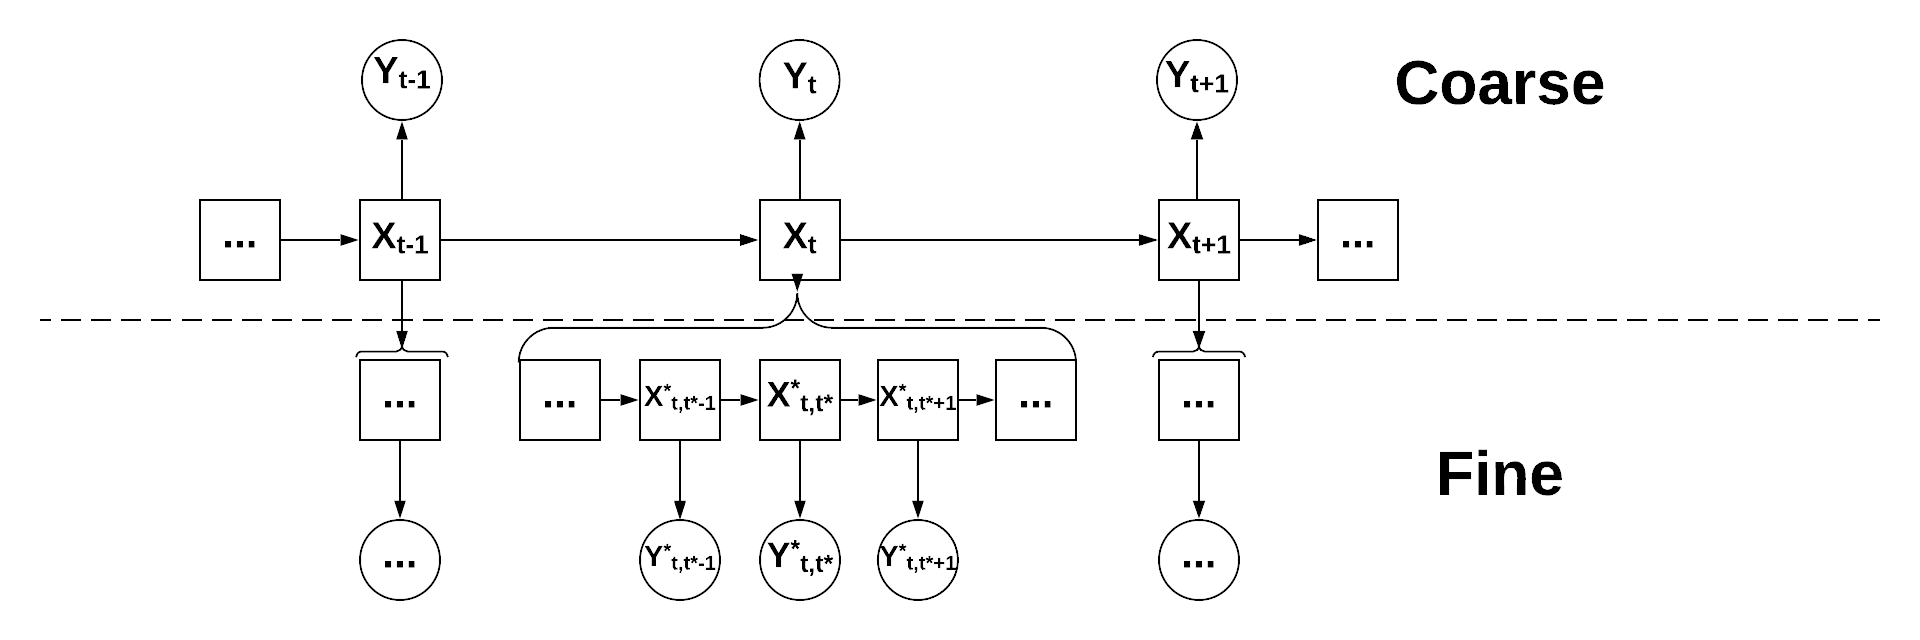
\includegraphics[width=3.75in]{../Plots/HHMM.png}  
      \label{fig:HHMM}
    \end{subfigure}
    %
    \hrule
    %
    \begin{subfigure}{\textwidth}
      \centering
      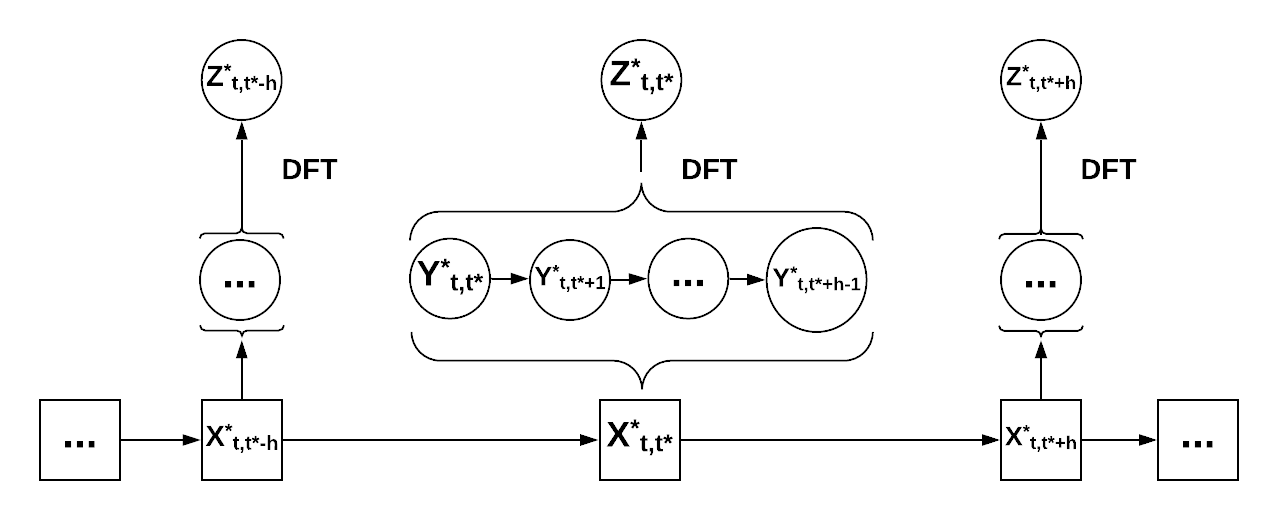
\includegraphics[width=3.5in]{../Plots/HMM-DFT.png}  
      \label{fig:HMM-DFT}
    \end{subfigure}
    \caption{Dependence structure of a standard HMM (top), CarHMM (middle-top), HHMM (middle-bottom), and HMM-DFT (bottom). Hidden state sequences are denoted by $X$ on the coarse scale and by $X^*$ on the fine scale. Observations are denoted by $Y$ on the coarse scale and by $Y^*$ on the fine scale. The coarse-scale process is not included in the HMM-DFT because moving window transformations often only apply to fine-scale data. The fine-scale observations of the HMM-DFT are transformed using a moving window and denoted by $\Z$ with corresponding fine-scale hidden states $\tilde X^*$.}
    \label{fig:models}
\end{figure}

%%% data %%%

\begin{figure}[ht]
	\centering
	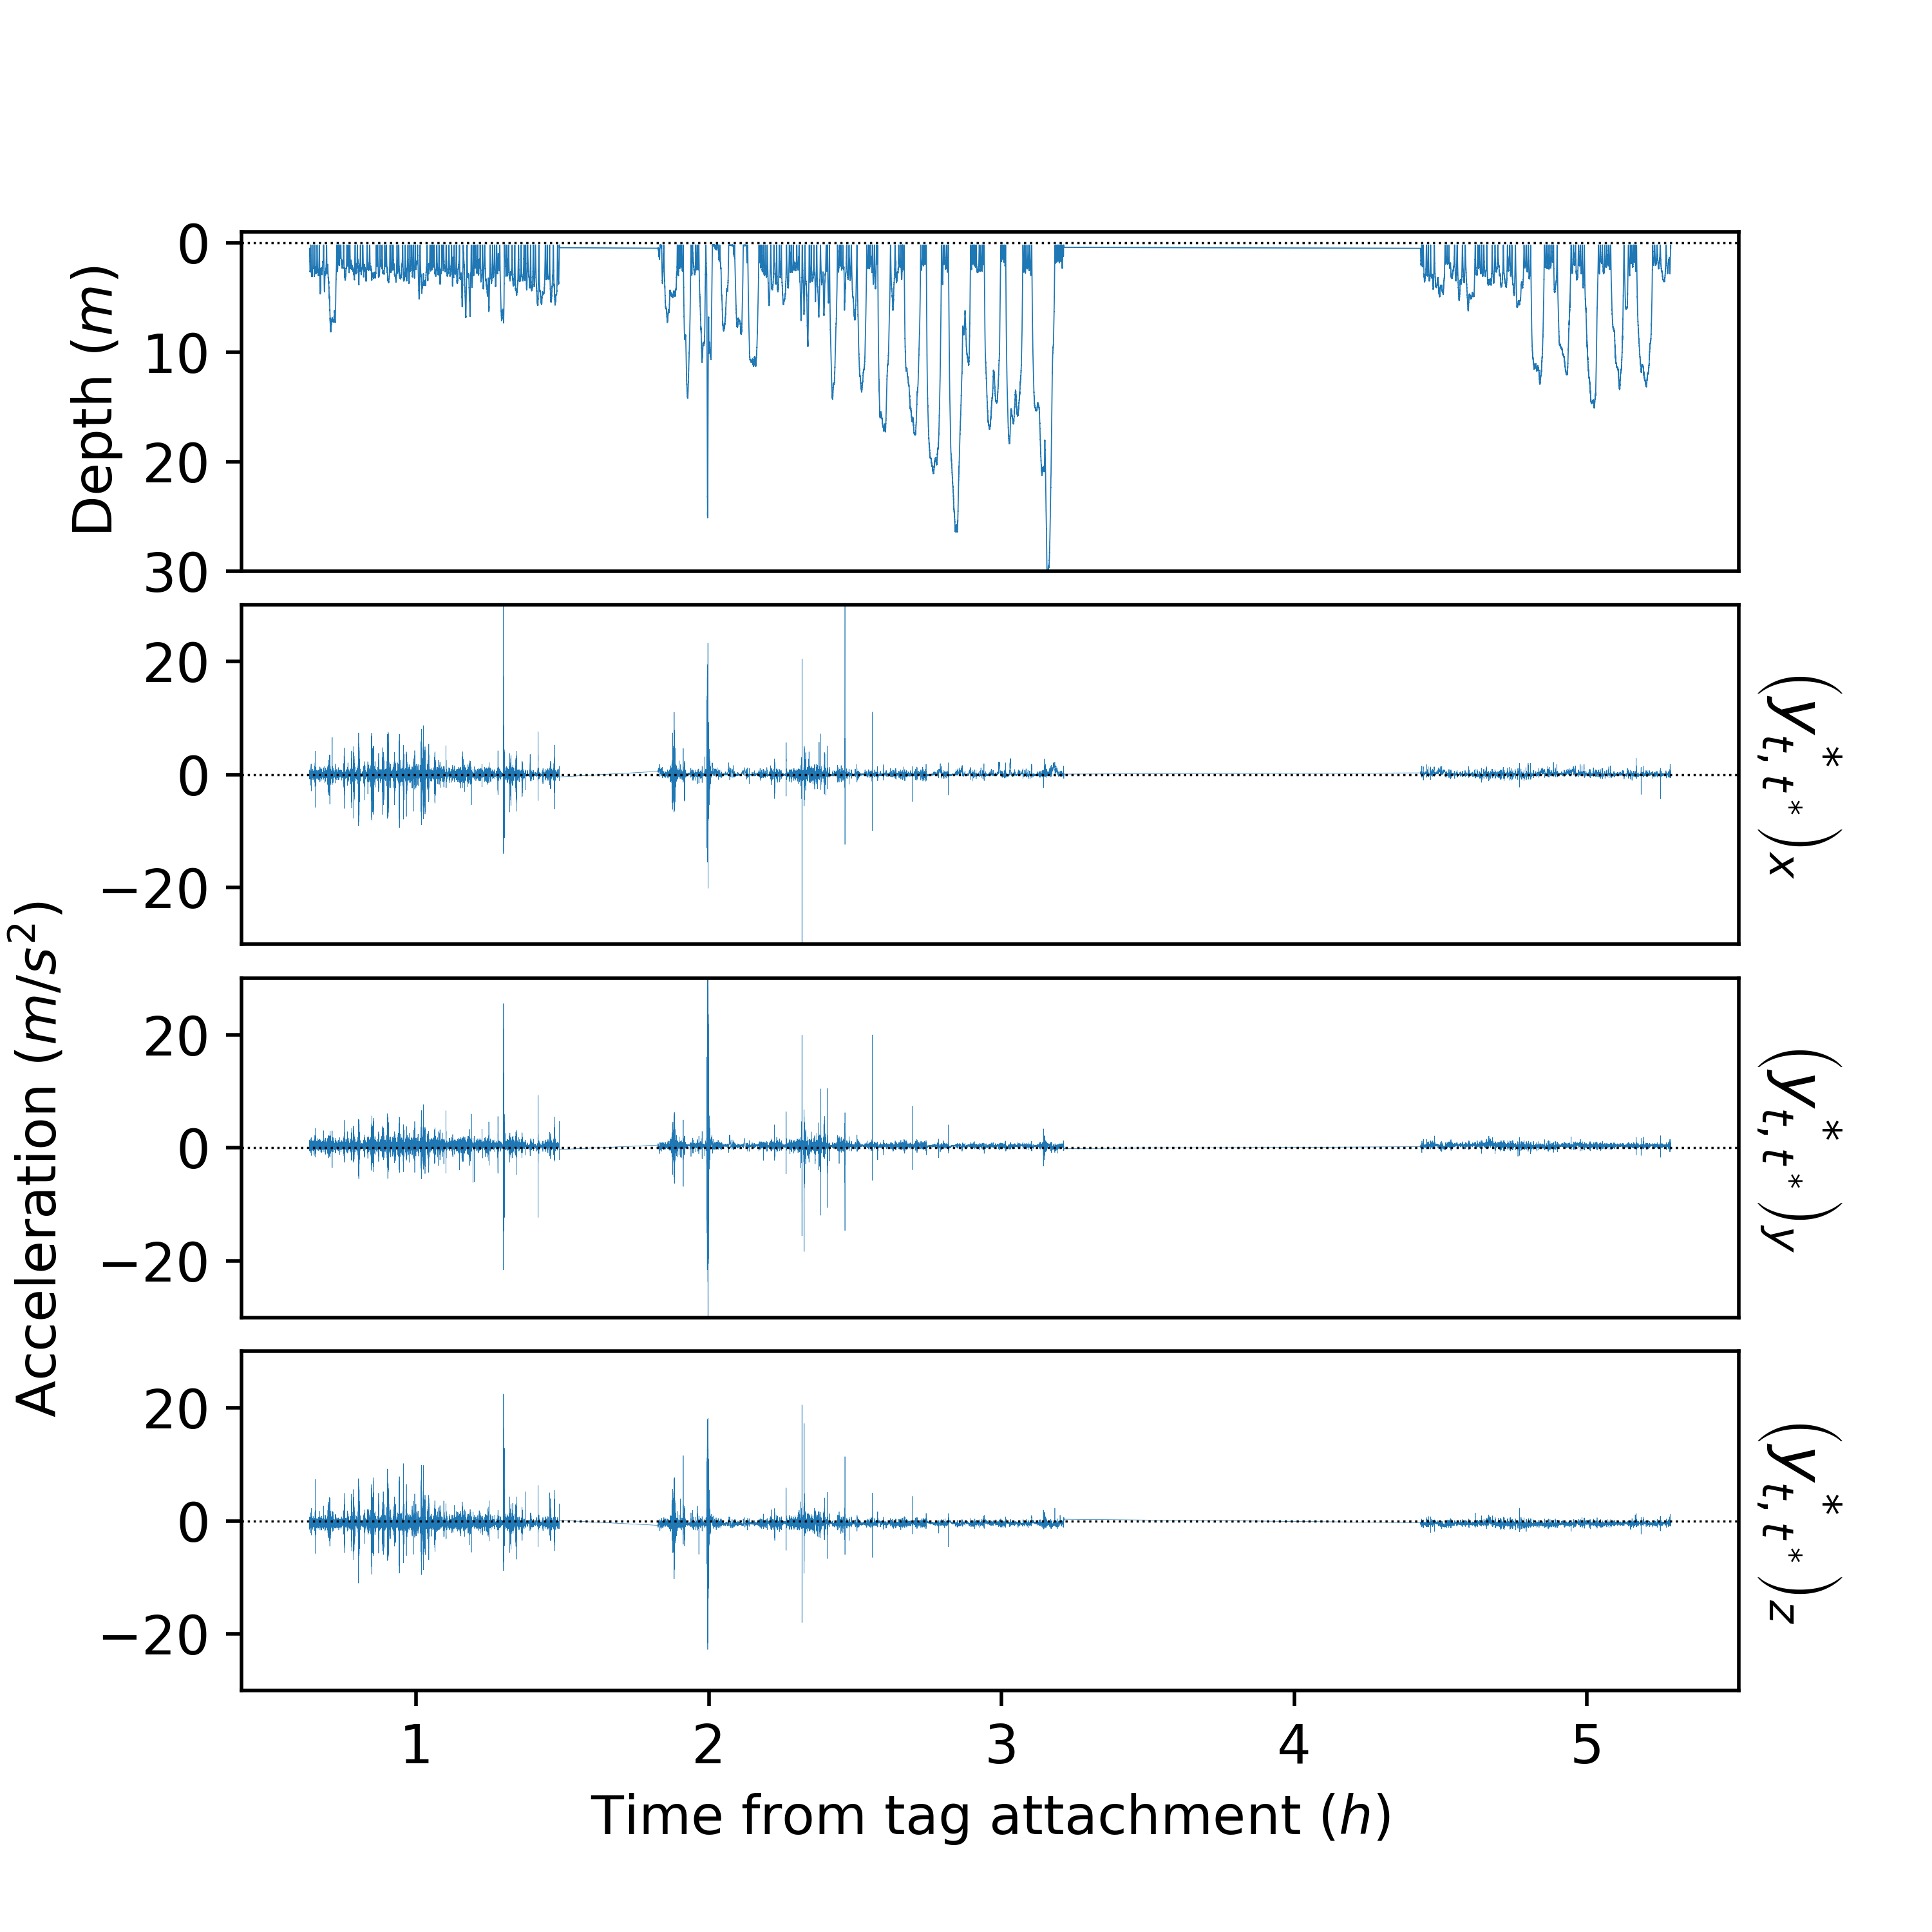
\includegraphics[width=5.25in]{../Plots/2019/20190902-182840-CATs_OB_1_0_267_CarHHMM2_raw_data.png}
	\caption{Dive depth (top panel) and three-dimensional acceleration (bottom three panels) from a killer whale over approximately 5 $h$. An exact physical interpretation of each component of acceleration is difficult due to variations in tag orientation. There are data gaps occurring from around hours $1.5$ to $1.8$ and from around hours $3.2$ to $4.5$. Both data gaps are excluded from analyses.}
	\label{fig:data}
\end{figure}

%%% Case Study %%%

\begin{figure}[ht]
	\centering
	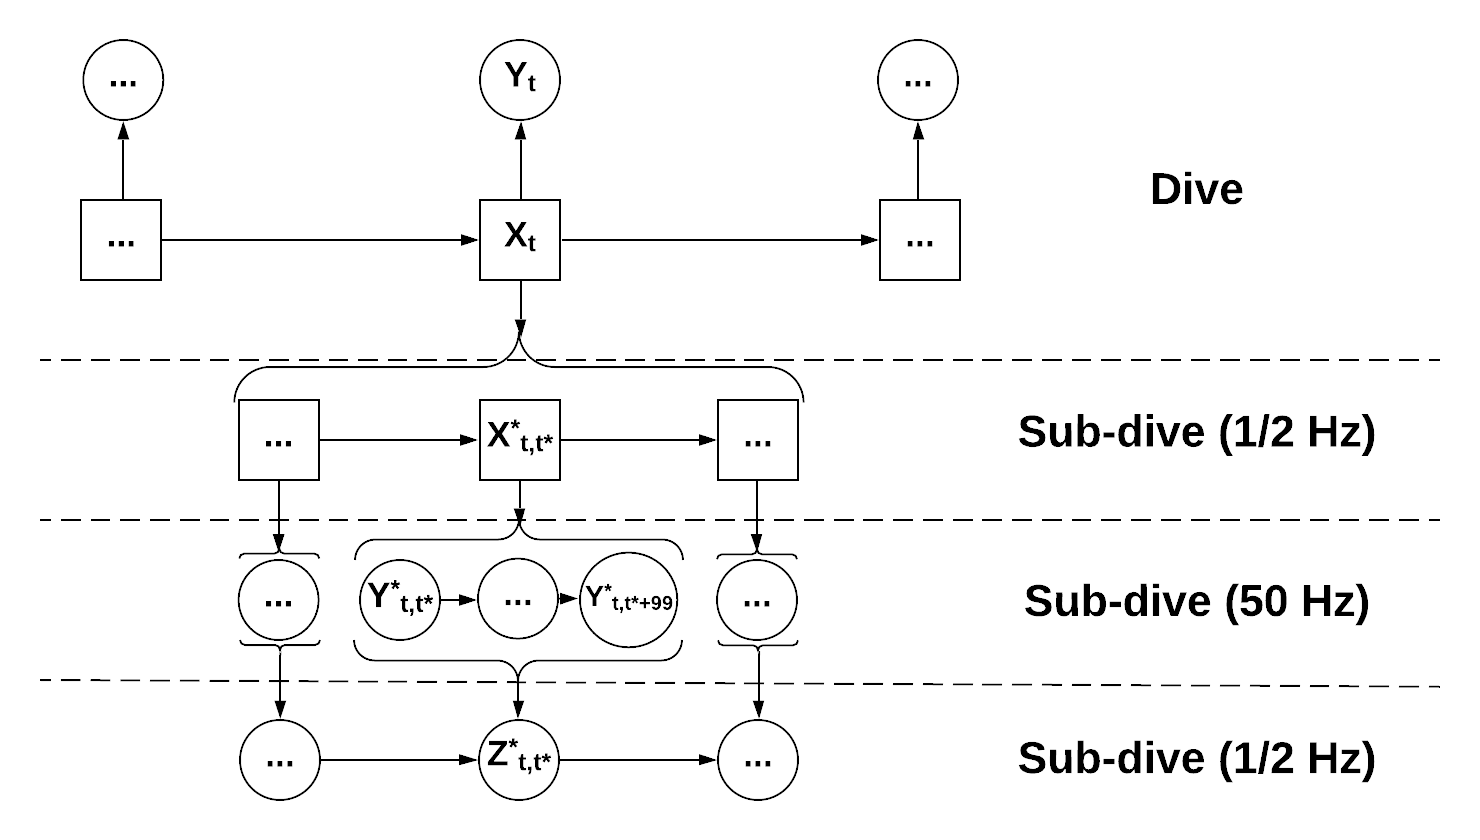
\includegraphics[width=5in]{../Plots/CarHHMM-DFT.png}
	\caption{Graphical representation of the CarHHMM-DFT used in the simulation and case studies. The type of dive $t$ is denoted by $X_t$, and $Y_t$ represents the associated dive duration. The raw acceleration vector associated with dive $t$ and time stamp $t^*$ is denoted by $Y^*_{t,t^*}$. The subdive state of the killer whale during dive $t$ and window $\tilde t^*$ is denoted by $\tilde X^*_{t,\tilde t^*}$, and the corresponding transformed observation is denoted by $\Z_{t,\tilde t^*}$.}
	\label{fig:CarHHMM-DFT}
\end{figure}

\begin{figure}[ht]
    \begin{subfigure}{\textwidth}
    	\centering
    	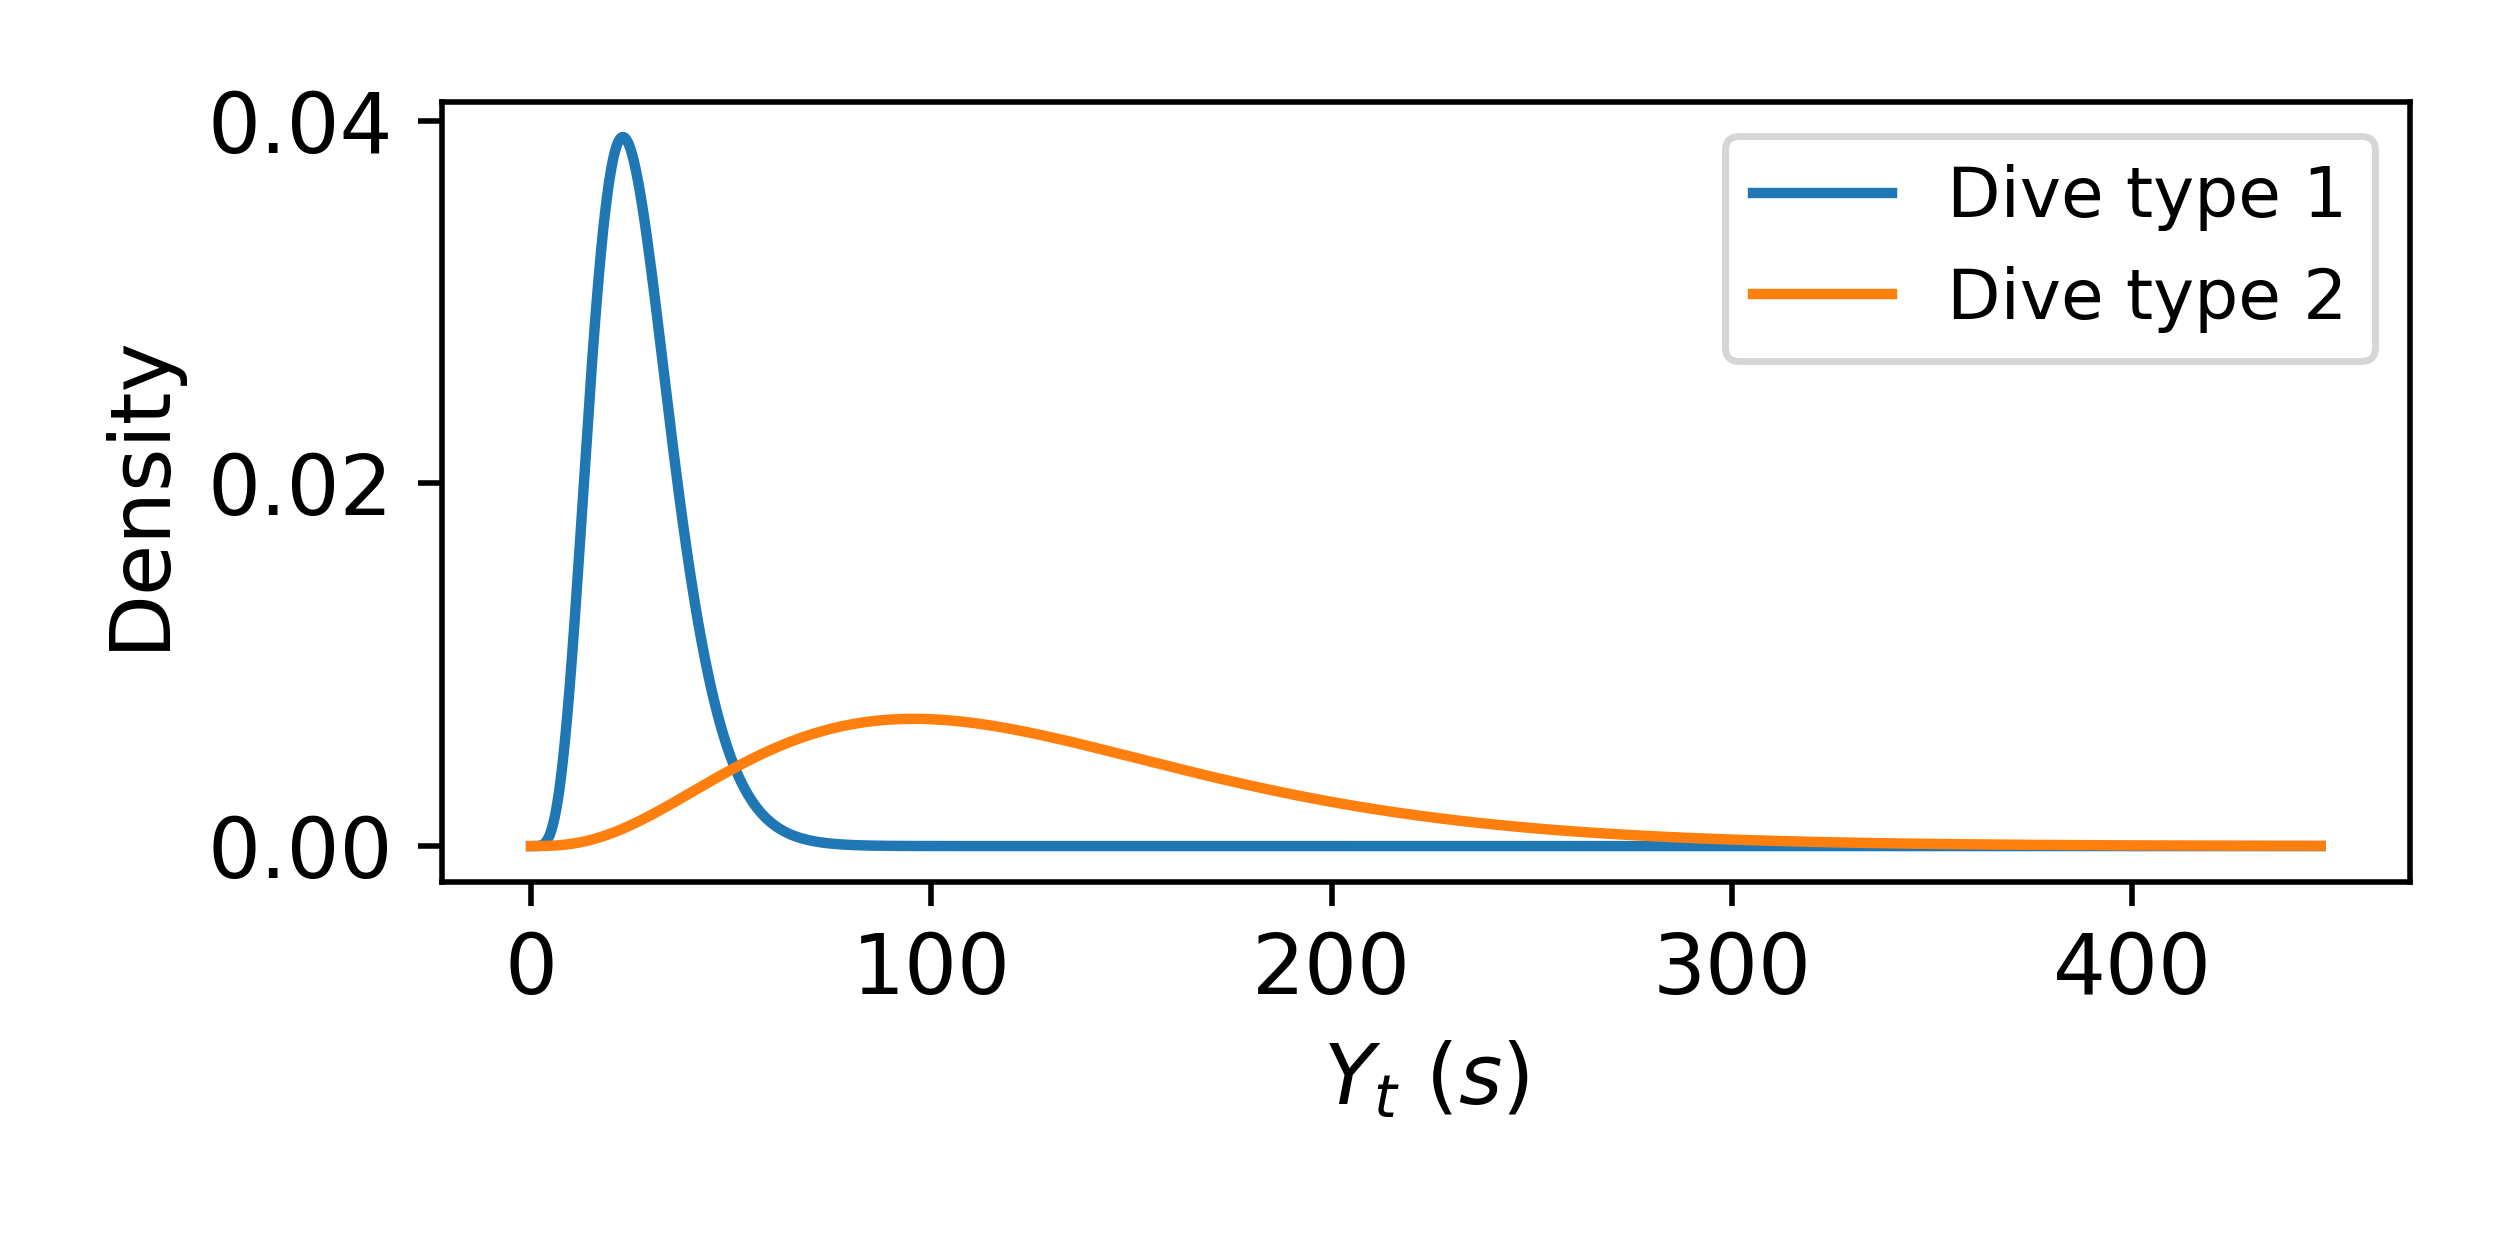
\includegraphics[width=3.5in]{../Plots/2019/20190902-182840-CATs_OB_1_0_267_CarHHMM2-coarse-emissions.png}
    \end{subfigure}
    \newline
    \begin{subfigure}{\textwidth}
    	\centering
    	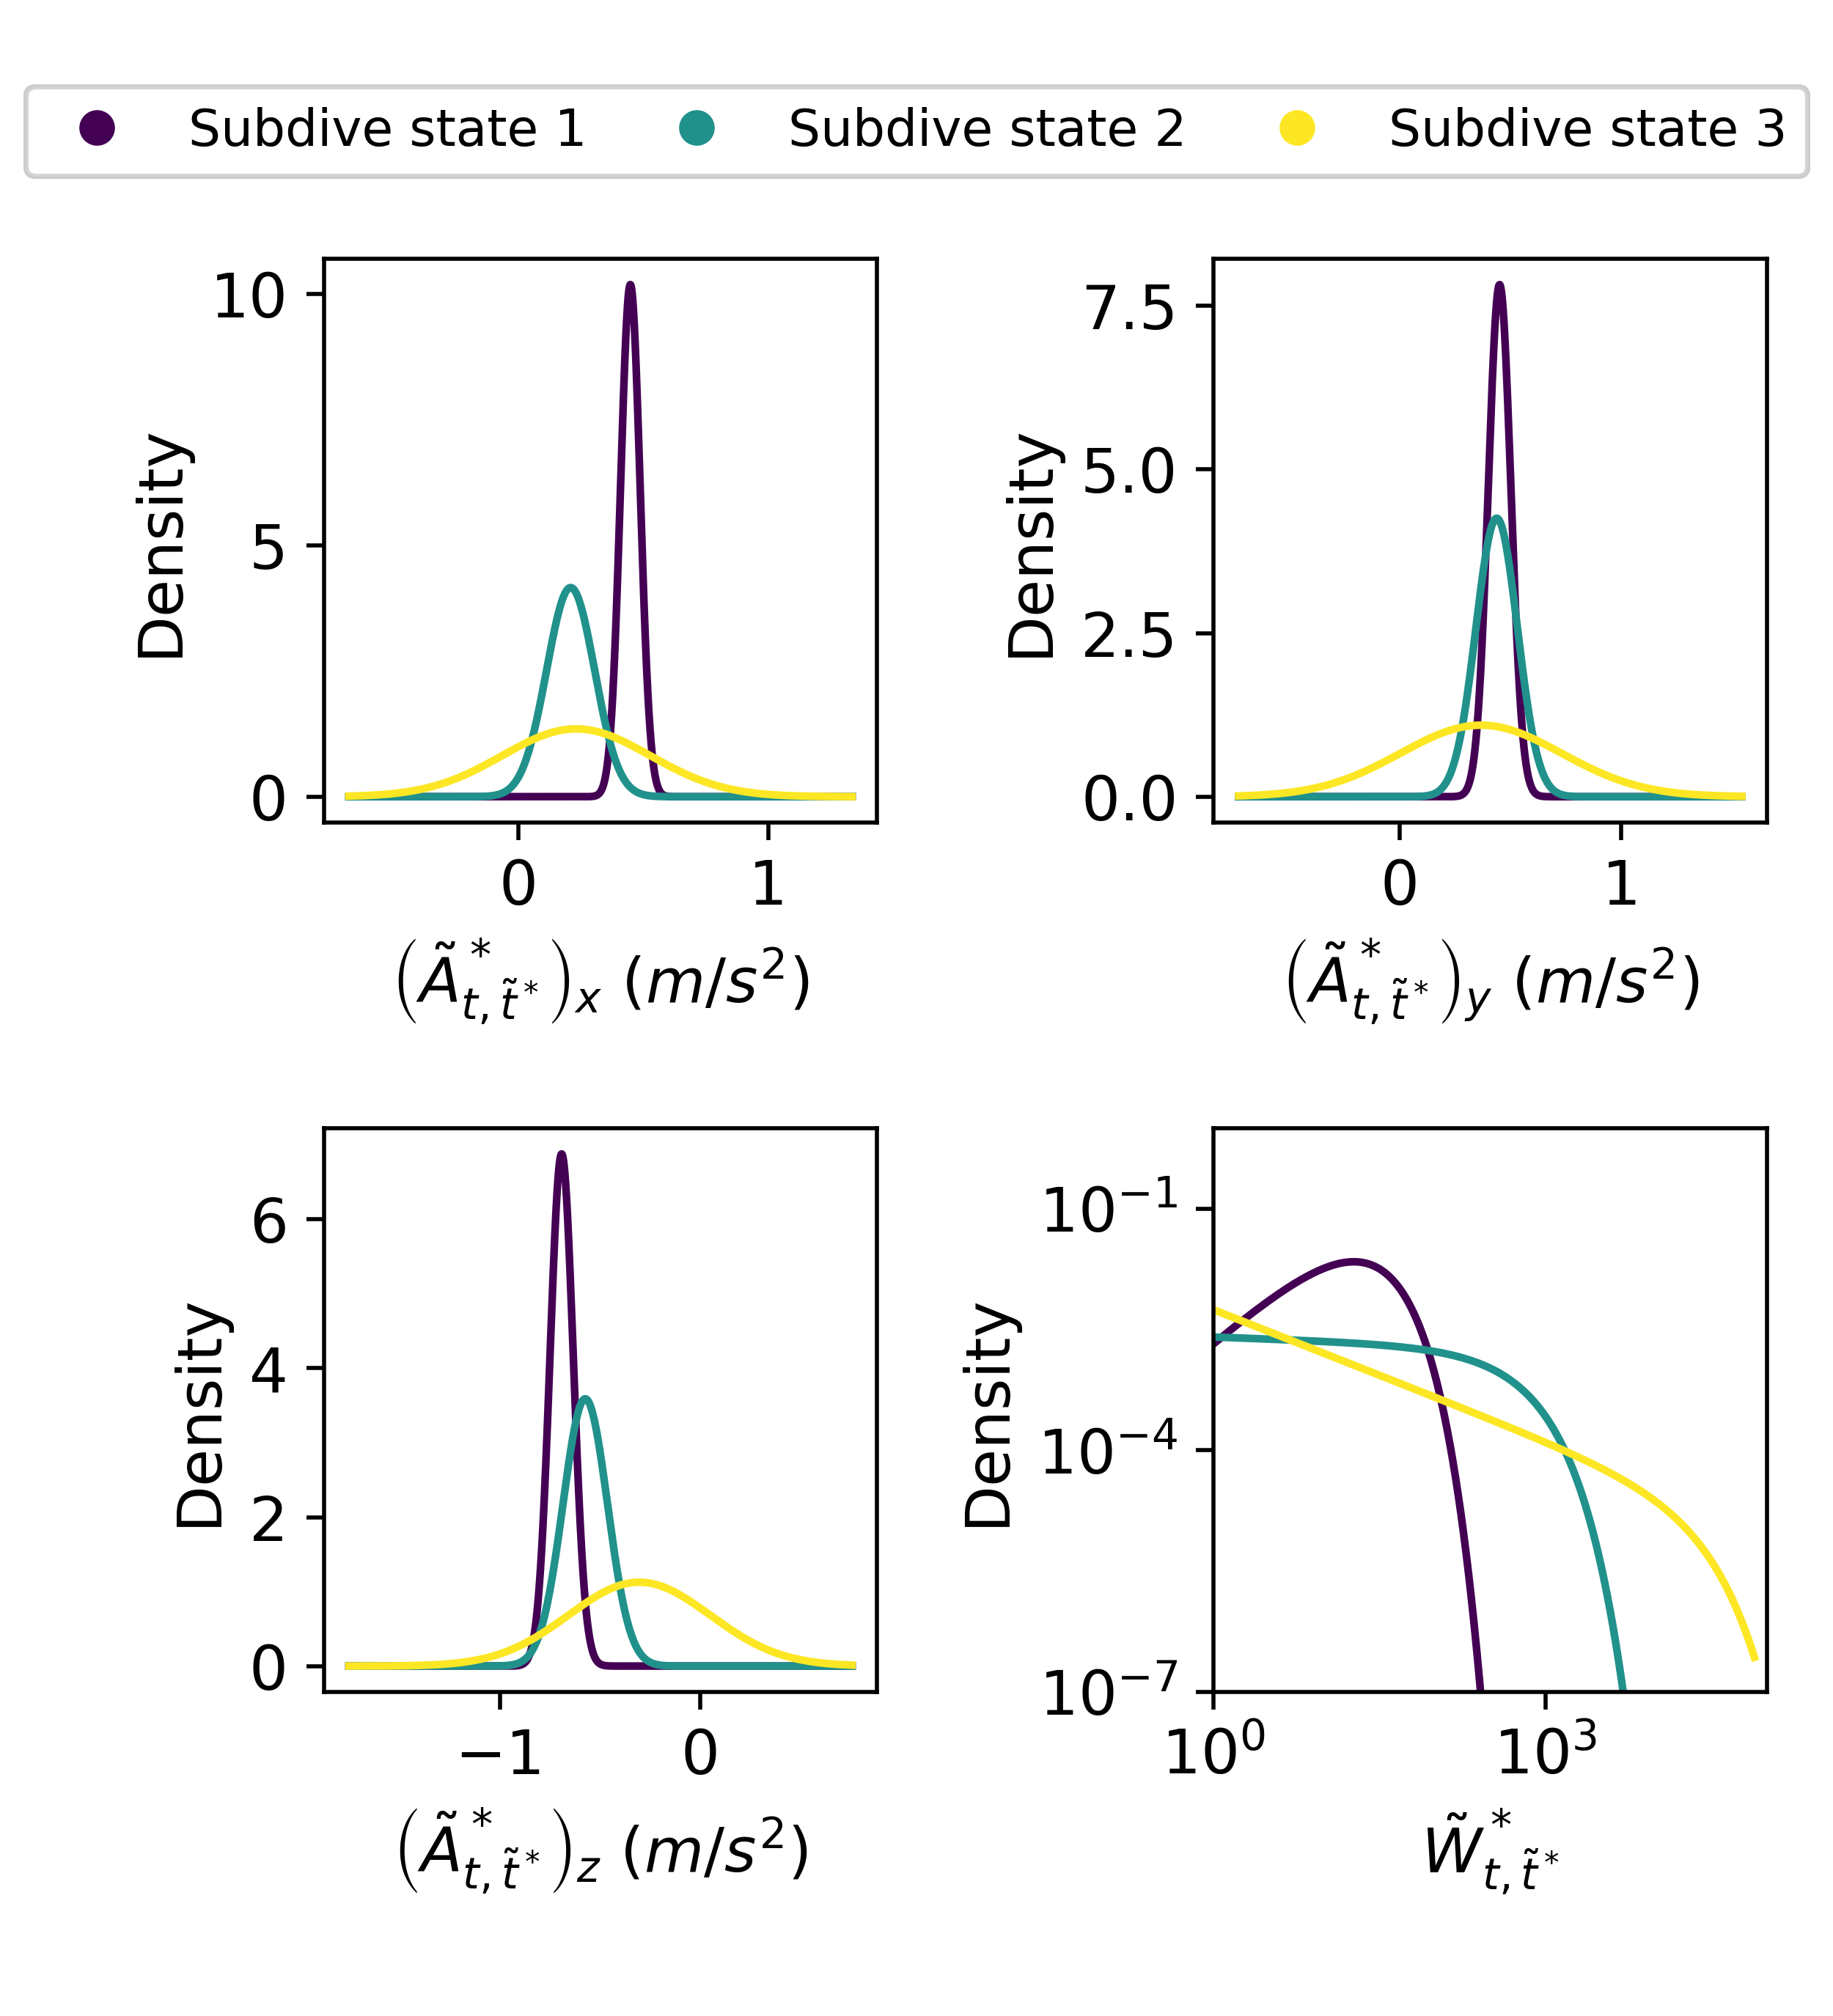
\includegraphics[width=3.5in]{../Plots/2019/20190902-182840-CATs_OB_1_0_267_CarHHMM2-fine-emissions.png}
    \end{subfigure}
    \caption{Estimated gamma densities of killer whale dive duration ($Y_t$) (top), estimated normal conditional densities of killer whale acceleration $(\Zone_{t,\tilde t^*} \mid \Zone_{t,\tilde t^*-1} = \mu_A^{*(\cdot,i^*)})$ (middle and bottom left), and estimated gamma densities of ``wiggliness" $(\Ztwo_{t,\tilde t^*})$ plotted on a log-log scale (bottom right). The densities of $Y_t$ correspond to dive types 1 and 2, while the densities of $\Zone_{t,\tilde t^*}$ and $\Ztwo_{t,\tilde t^*}$ correspond to subdive states 1, 2, and 3. The densities are estimated by fitting the CarHHMM-DFT to the case study data (see Table \ref{table:emis_dists_CarHHMM-DFT}).}
    \label{fig:emis}
\end{figure}

\begin{figure}[ht]
	\centering
	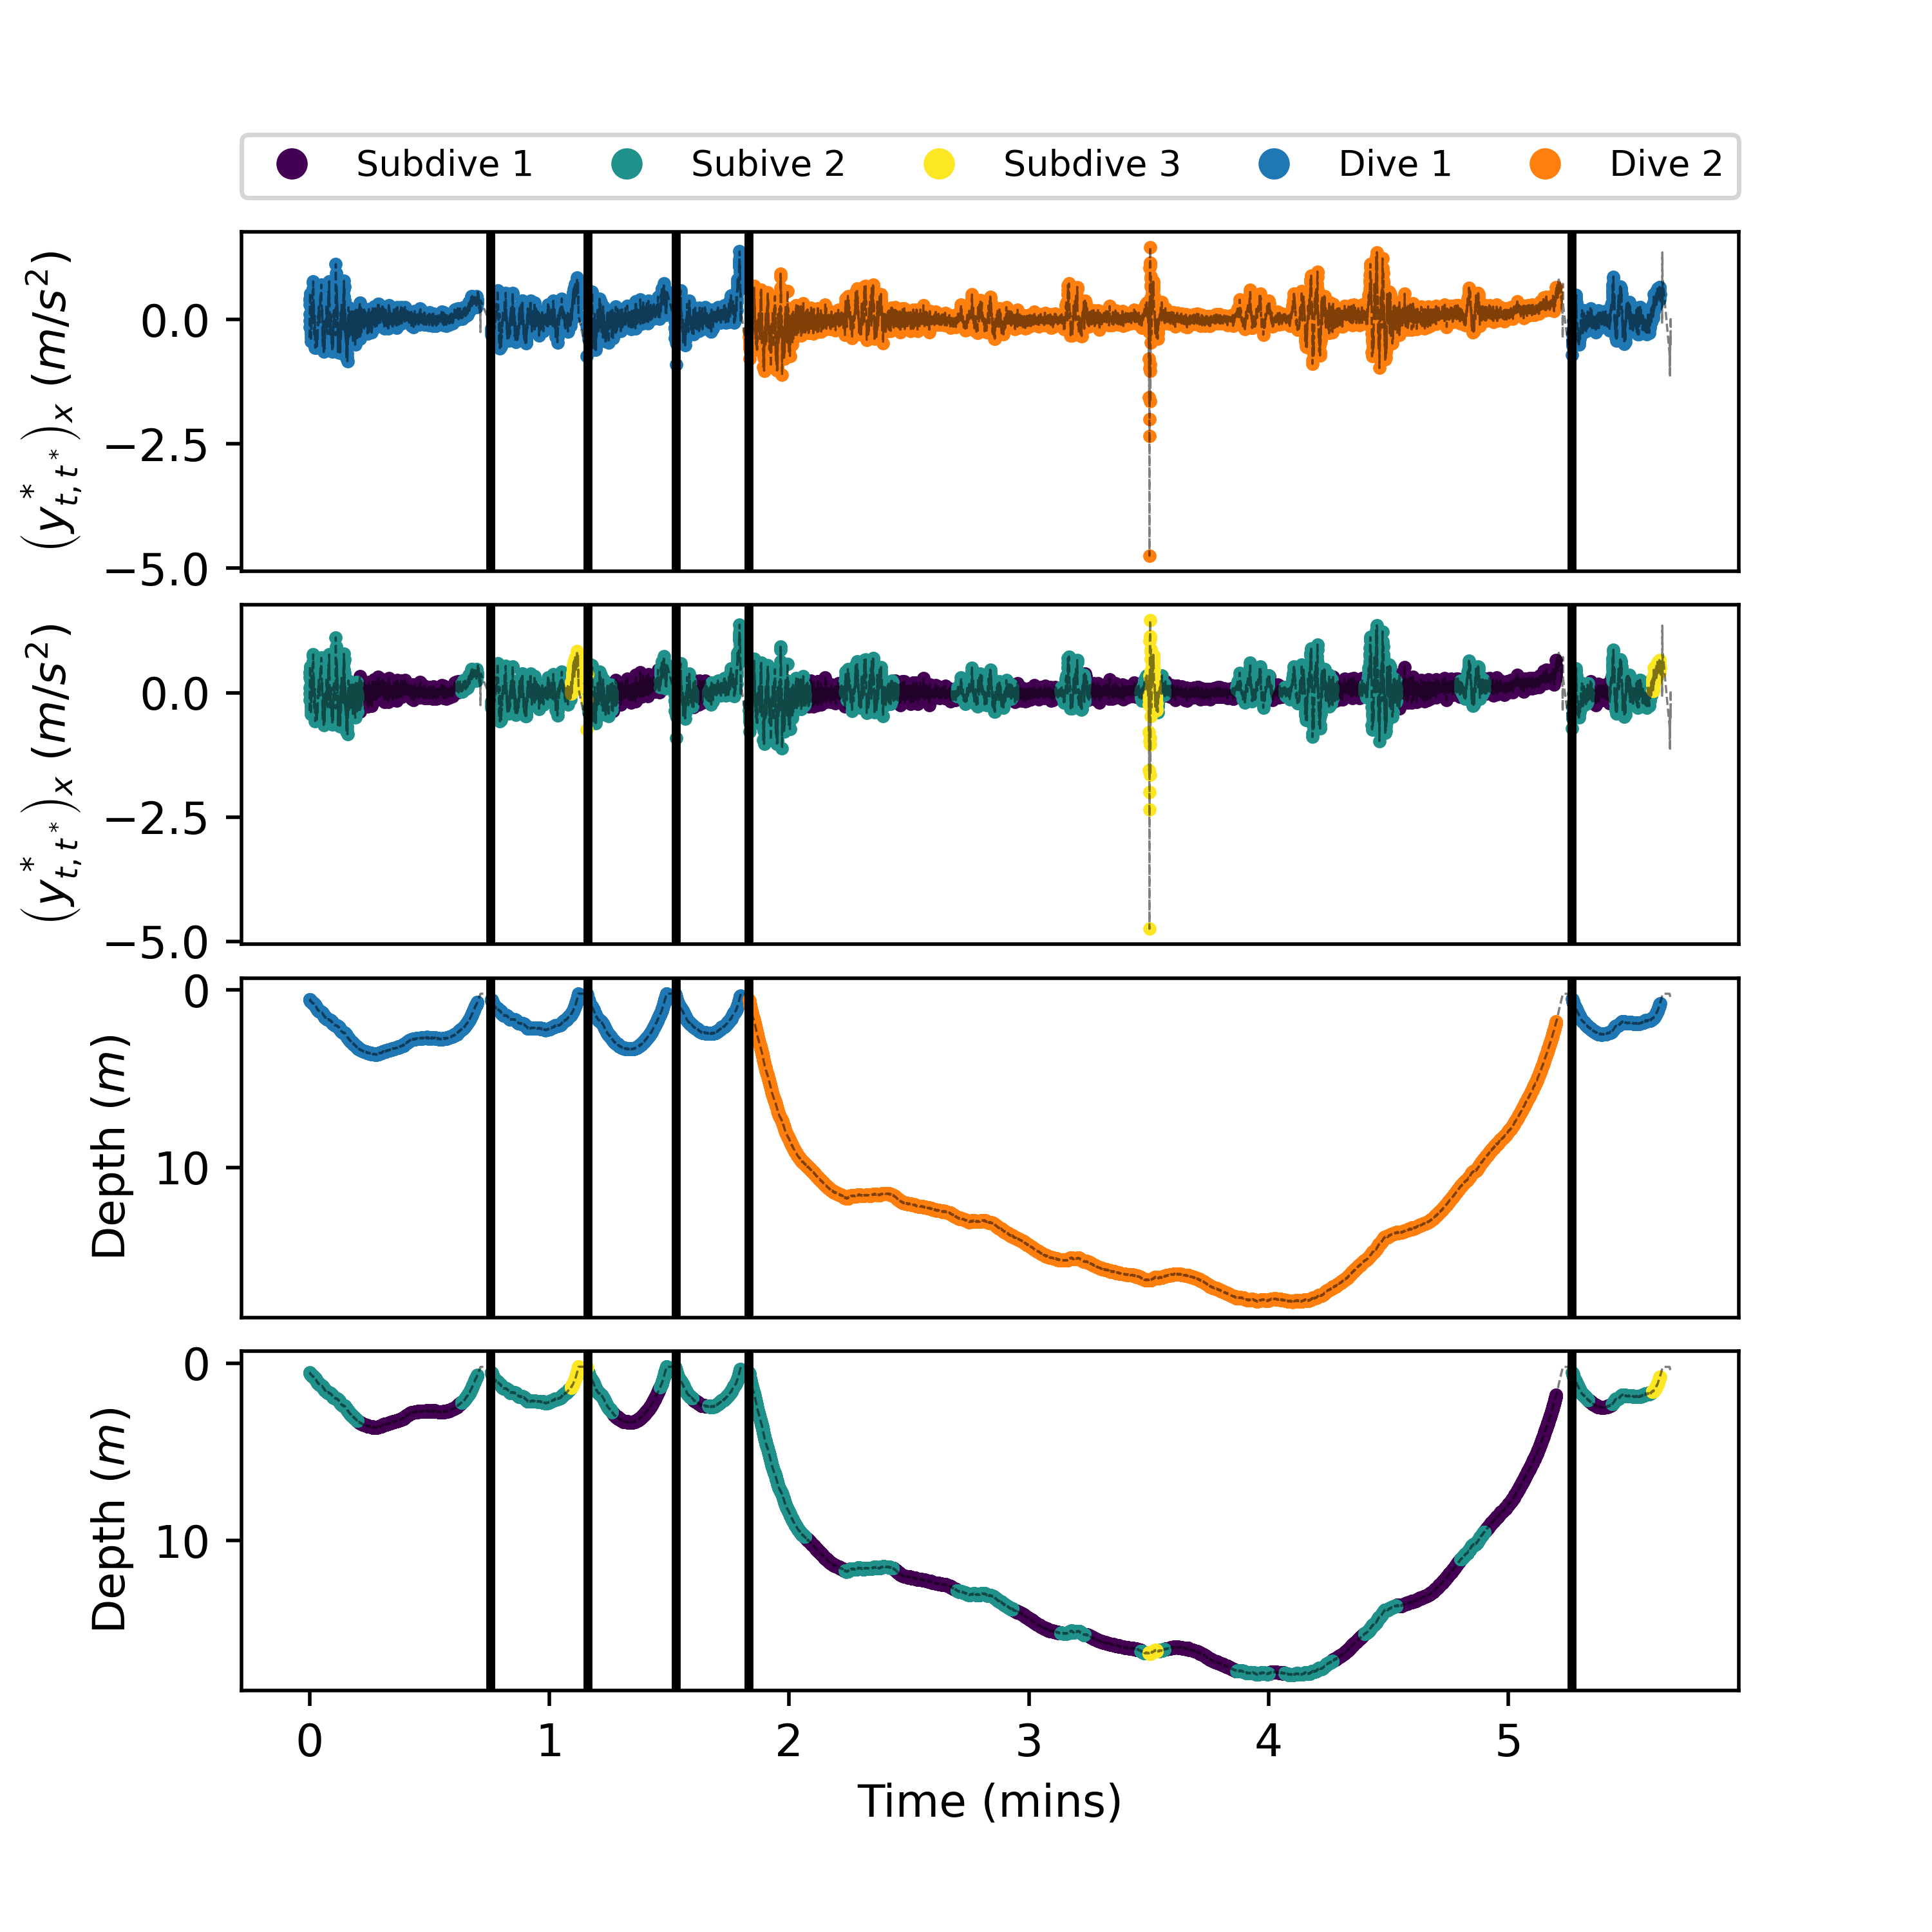
\includegraphics[width=4.75in]{../Plots/2019/20190902-182840-CATs_OB_1_0_267_CarHHMM2_decoded_dives.png}
	\caption{The $x$-component of acceleration, $(y^*_{t,t^*})_x$ (top two panels), and dive depth (bottom two panels) of a northern resident killer whale for a sequence of six selected dives. Each panel is partitioned into dives by vertical black lines. Curve colour in the first and third panels corresponds to estimated dive type while curve colour in the second and fourth panels corresponds to the estimated subdive state. Both dive type and subdive state are estimated by fitting the CarHHMM-DFT to the data and applying the forward--backward algorithm to determine the hidden state with the highest probability.}
	\label{fig:labeled_dives}
\end{figure}

\begin{figure}[ht]
    \begin{subfigure}{0.45\textwidth}
    	\centering
    	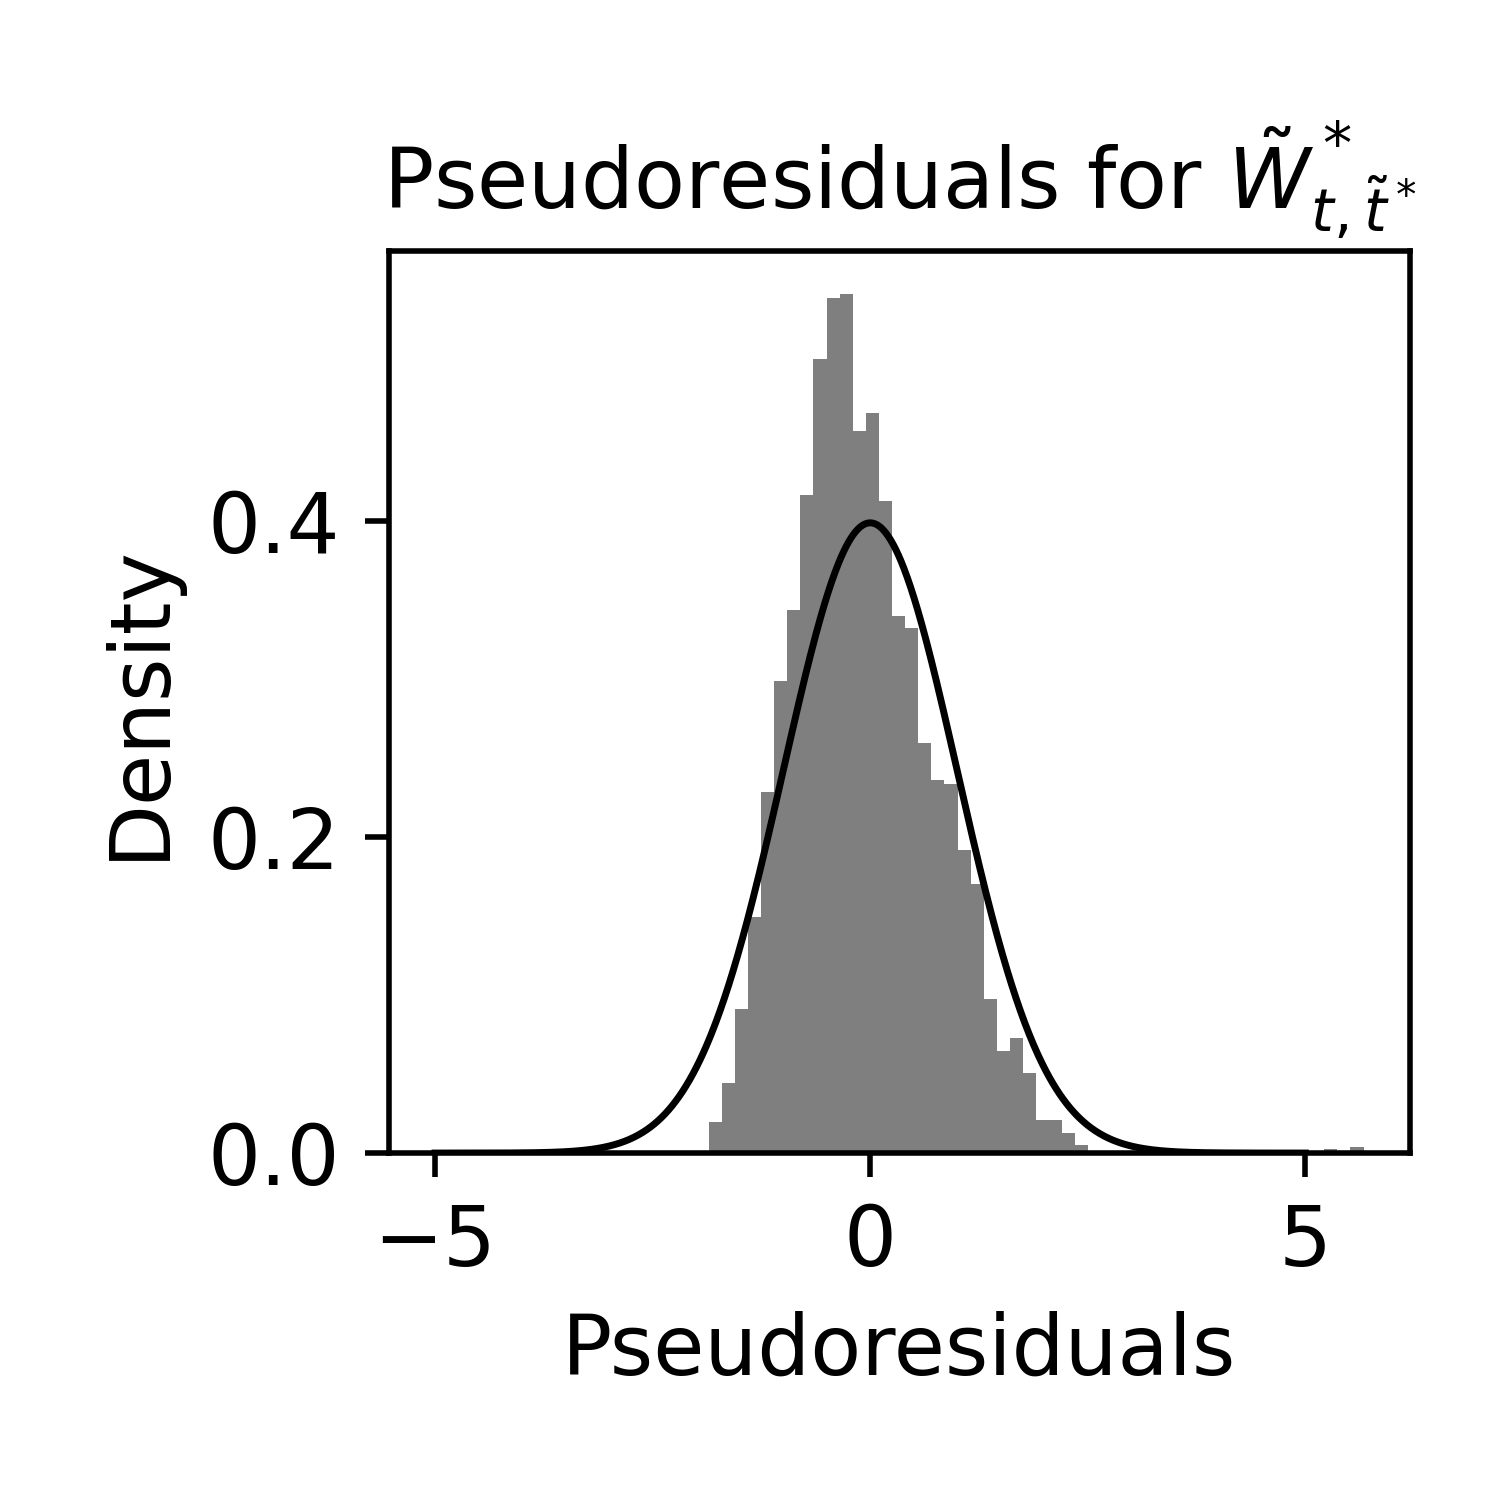
\includegraphics[width=2.25in]{../Plots/2019/20190902-182840-CATs_OB_1_0_267_CarHHMM2_pseudresids_ahat.png}
    \end{subfigure}
    \begin{subfigure}{0.45\textwidth}
    	\centering
    	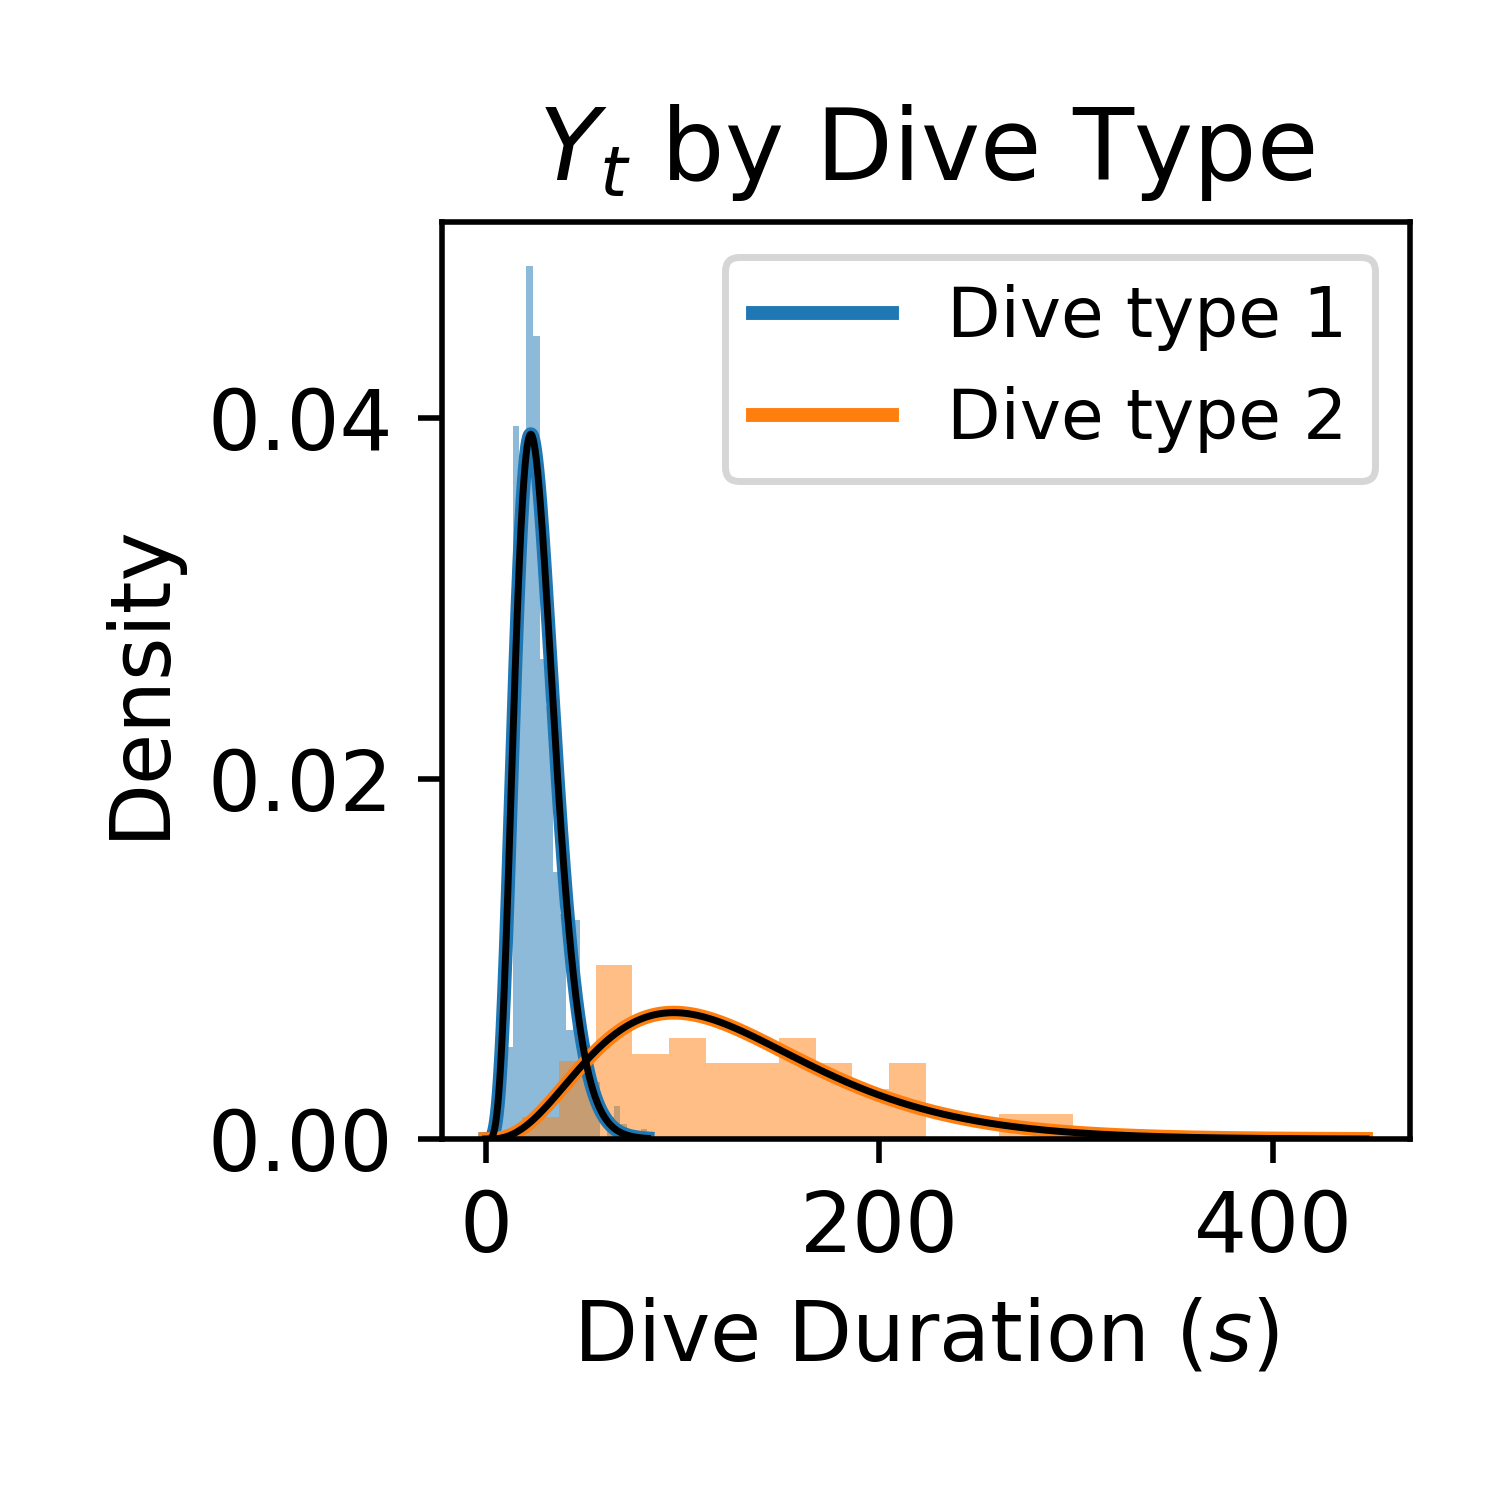
\includegraphics[width=2.25in]{../Plots/2019/20190902-182840-CATs_OB_1_0_267_CarHHMM2_empirical_hist_dive_duration.png}
    \end{subfigure}
    \caption{Pseudoresiduals of ``wiggliness"
    %$\left(\Phi^{-1} \left(\Pr(\Ztwo_{t,\tilde t^*} < \ztwo_{t,\tilde t^*}\big|Y,\tilde Y^* / \{\Ztwo_{t,\tilde t^*}\}) \right), \enspace \text{left} \right)$
    plotted over a standard normal density (left) and weighted empirical distributions of dive duration $Y_t$ plotted over the corresponding fitted gamma distributions (right). Both plots are generated by fitting the CarHHMM-DFT to the killer whale case study data and applying the forward--backward algorithm.}
    \label{fig:model_checking}
\end{figure}

%%% simulation study %%%

\begin{figure}[ht]
    \centering
    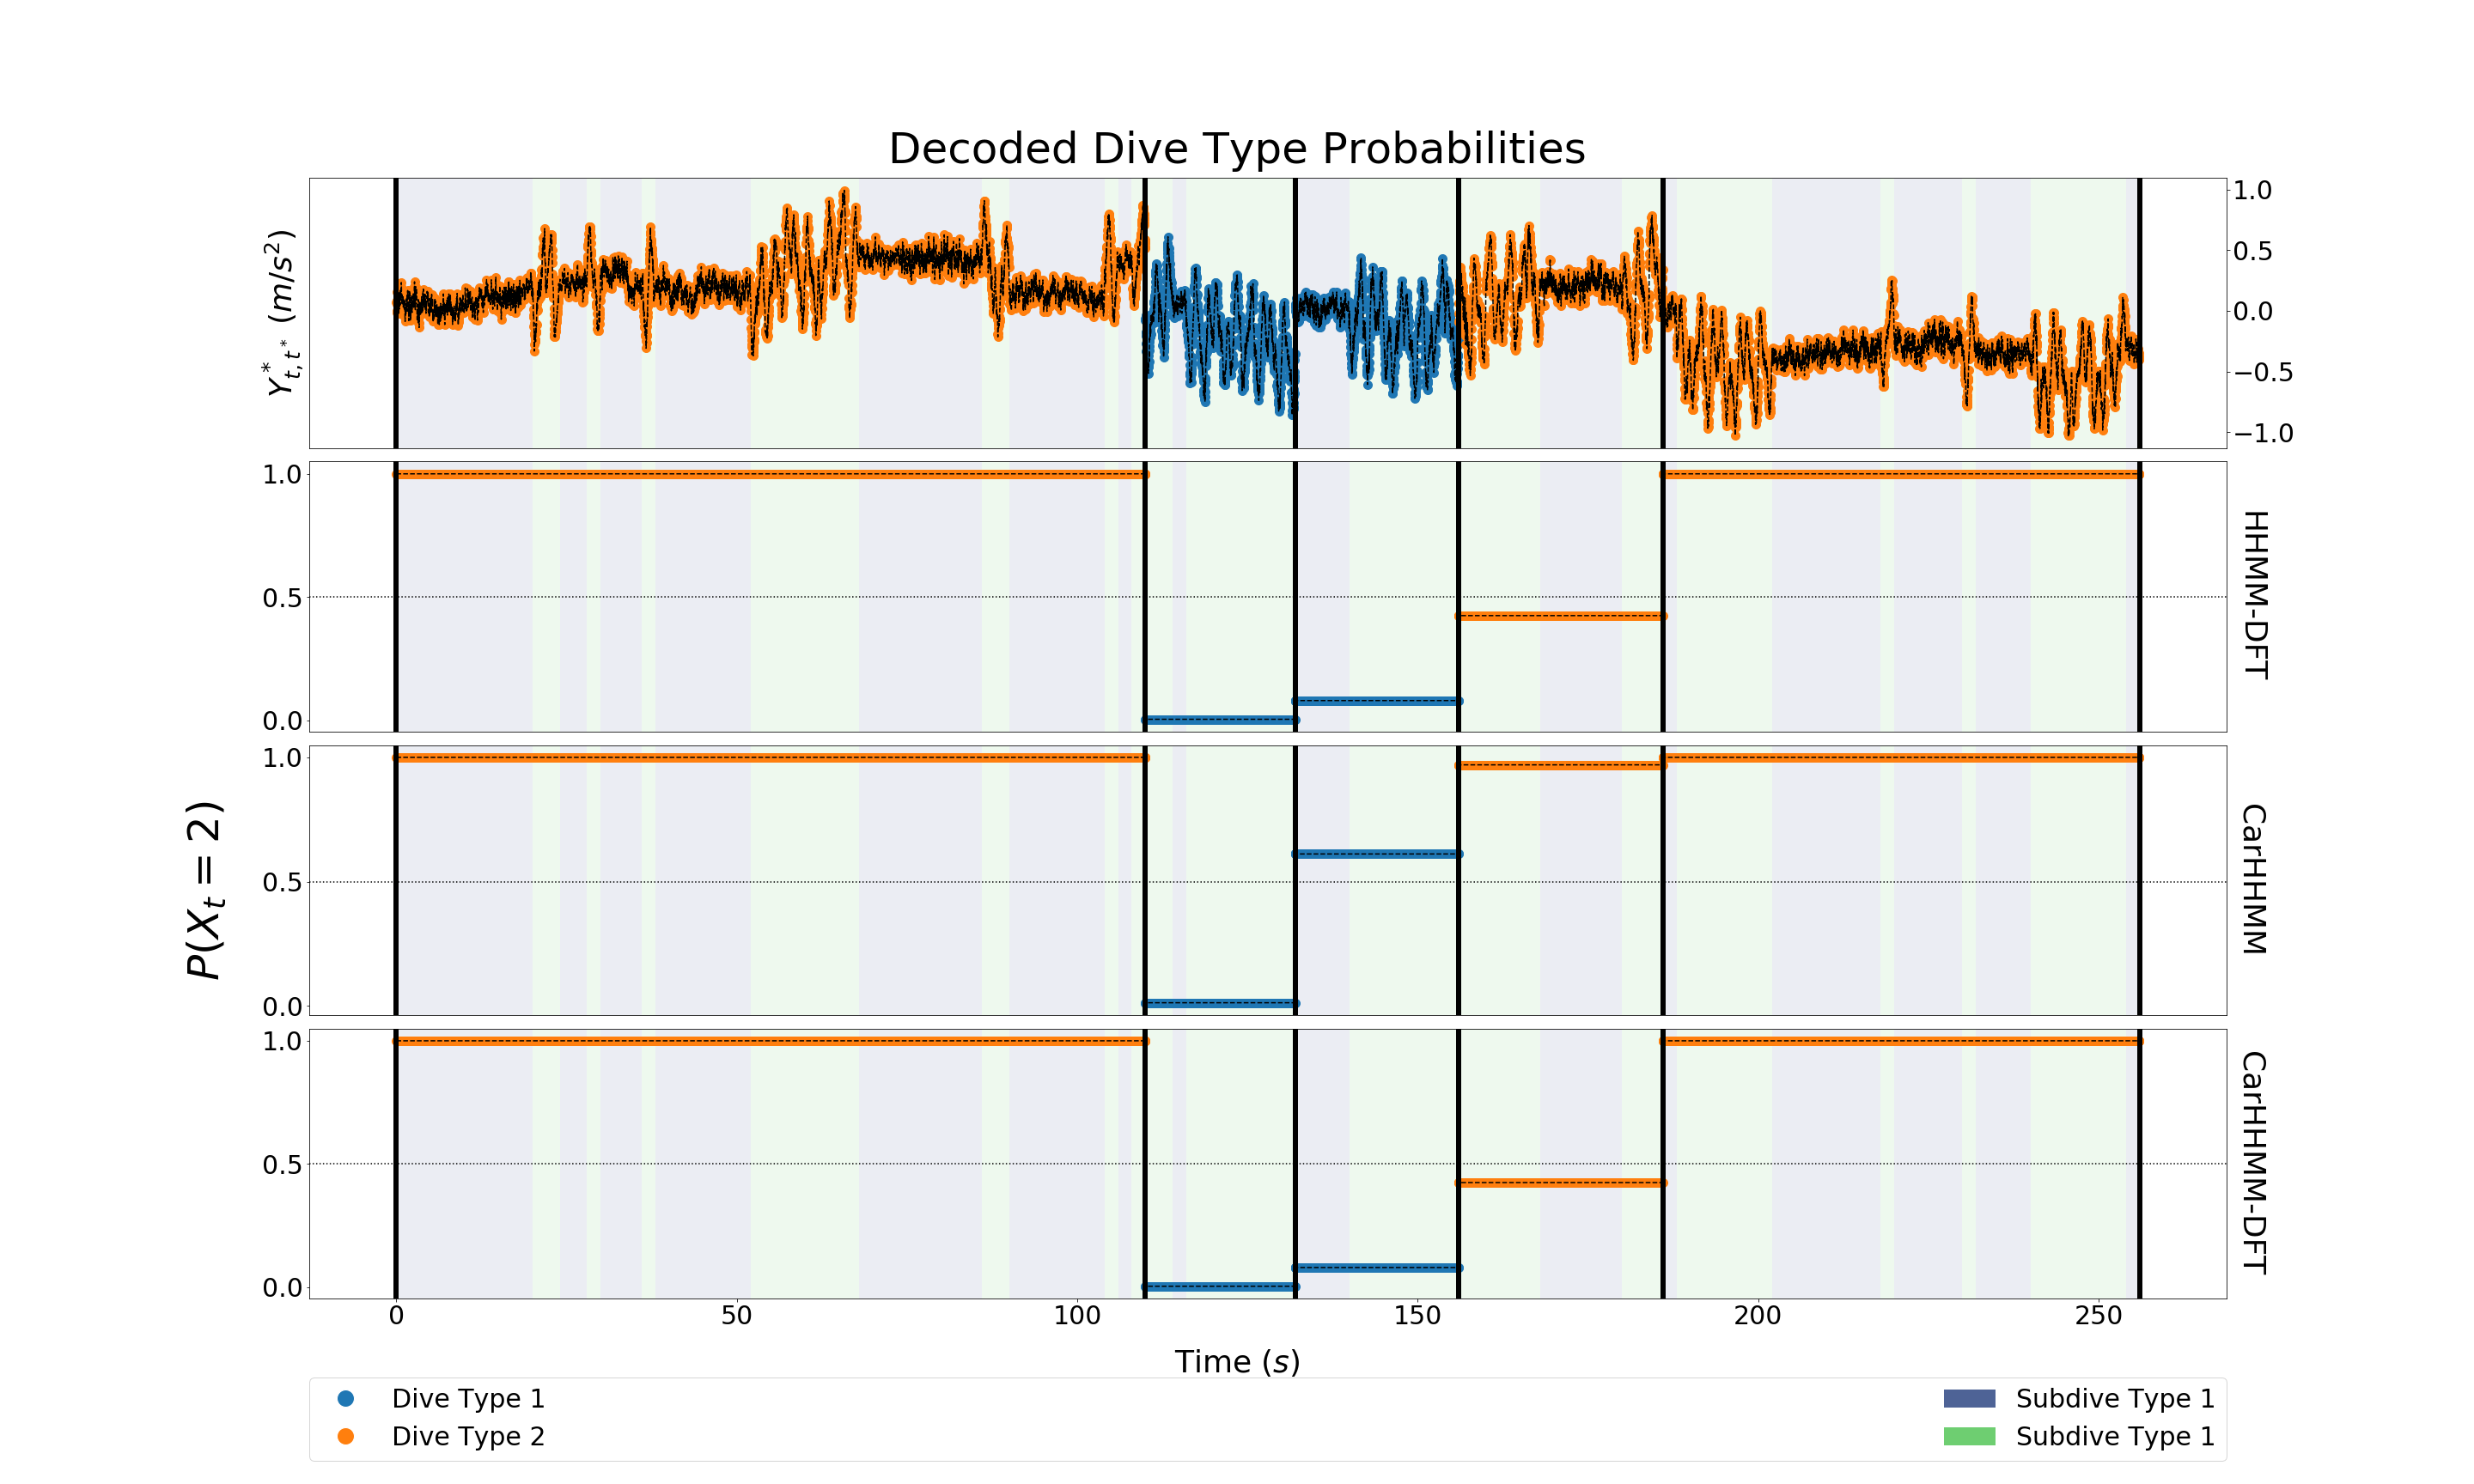
\includegraphics[width=4.5in]{../Plots/Posterior_Coarse_States.png}
    \caption{Estimated probabilities that each dive $t$ is of type $x_t$ for six selected dives of a simulated data set of killer whale dive behaviour. Each panel is partitioned into dives by vertical black lines. Curve colour corresponds to true dive type while background colour corresponds to true subdive state. The CarHMM-DFT is omitted because it assumes that there is only one dive type.}
    \label{fig:acc_coarse}
\end{figure}

\begin{figure}[ht]
    \centering
    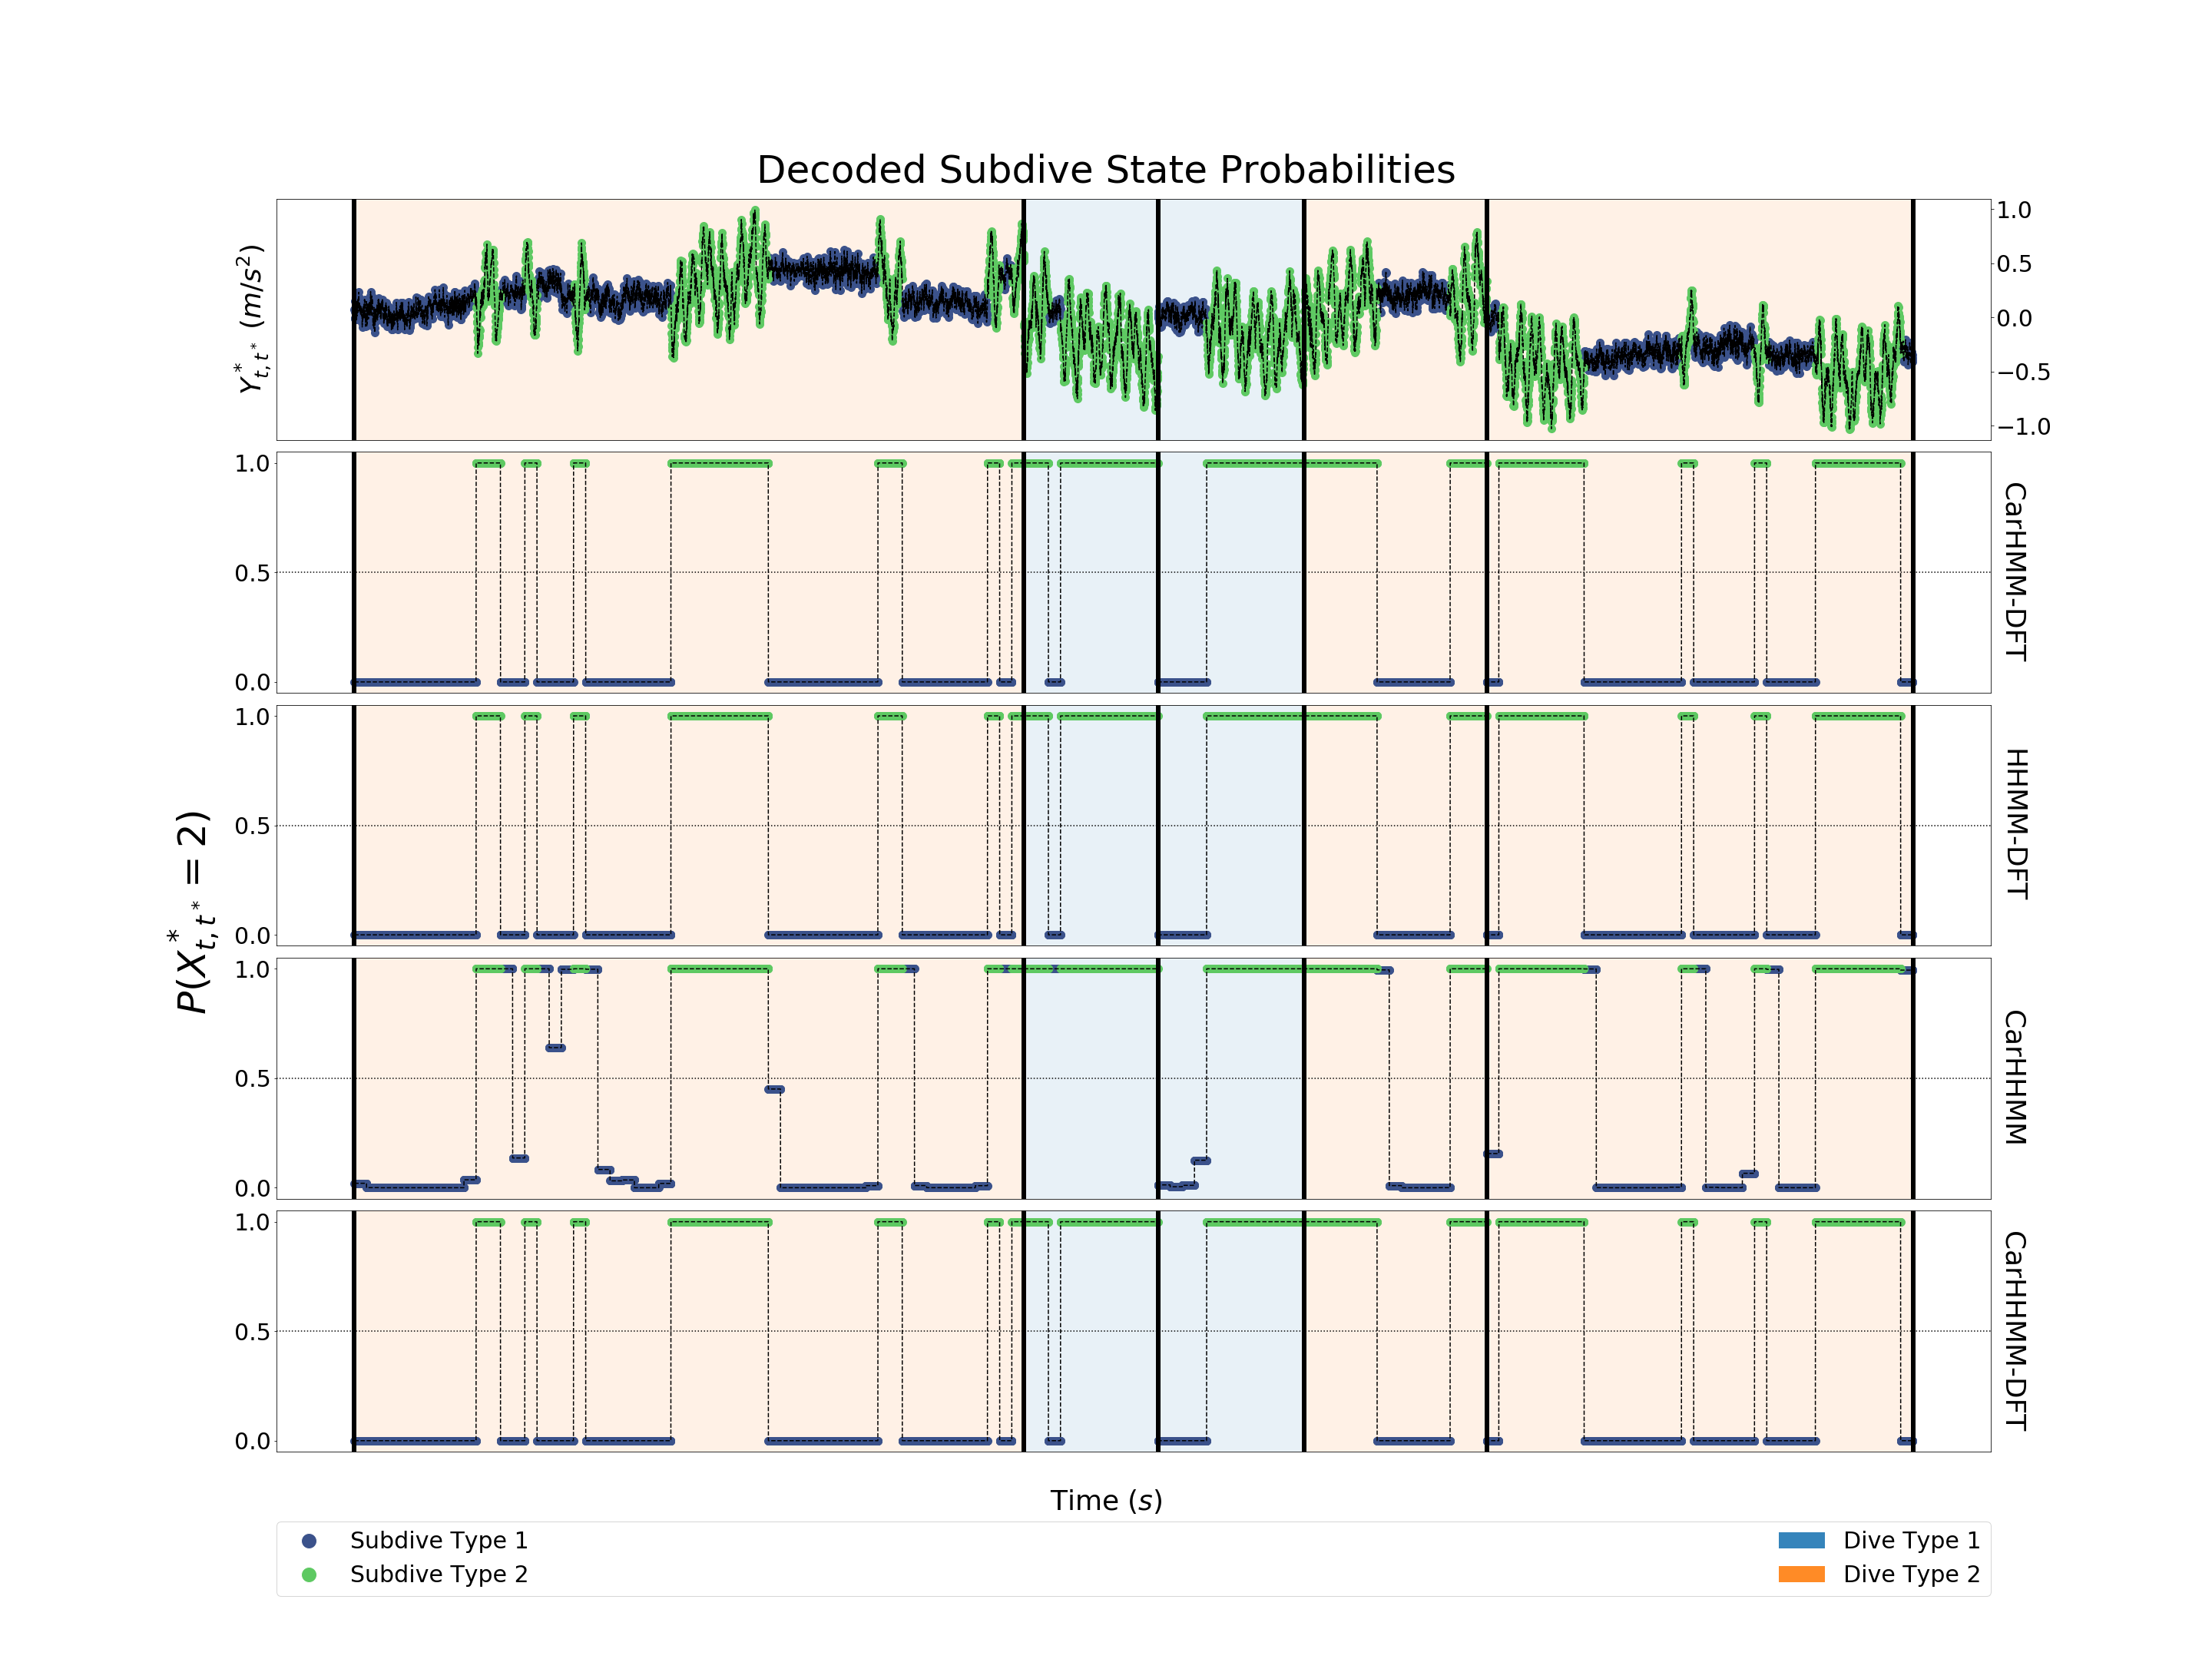
\includegraphics[width=4.5in]{../Plots/Posterior_Fine_States.png}
    \caption{Estimated probabilities that each window $(t,\tilde t^*)$ corresponds to subdive state $\tilde x^*_{t,\tilde t^*}$ for six selected dives of a simulated data set of killer whale dive behaviour. Each panel is partitioned into dives by vertical black lines. Curve colour corresponds to true subdive state while background colour corresponds to true dive type.}
    \label{fig:acc_fine}
\end{figure}